\documentclass[a4paper, 12pt]{article}
\usepackage[utf8]{inputenc}
\usepackage[french]{babel}
\usepackage[T1]{fontenc}
\usepackage[top=2cm,bottom=2cm,left=2cm,right=2cm]{geometry}
\usepackage{hyperref}
\usepackage{graphicx}
\usepackage{caption}
\usepackage{sectsty}
\usepackage{xcolor}
\usepackage{tabularx}
\usepackage{colortbl}
\usepackage{tkz-graph}
\usepackage{listings}
\usepackage[linesnumbered,ruled,french,onelanguage]{algorithm2e}
\usepackage{tikz}
\usepackage{fancyhdr}
\usepackage{float}


% Couleurs pour le thème clair des codes sources
\definecolor{fondCode}{HTML}{e6e6e6}
\definecolor{mots}{HTML}{A354BB}
\definecolor{string}{HTML}{50A14F}
\definecolor{commentaire}{HTML}{A1A2A8}
\definecolor{texte}{HTML}{383A42}

% Couleurs pour les codes du projet
\lstdefinestyle{styleCode}{
	backgroundcolor=\color{fondCode},
	commentstyle=\color{commentaire},
	keywordstyle=\color{mots},
	numberstyle=\fontsize{8}{10}\selectfont,
	stringstyle=\color{string},
	basicstyle=\color{texte}\ttfamily\footnotesize
}
% Pour les codes sources---------------------------------------------
\lstset{style=styleCode,
	breakatwhitespace=false,
	captionpos=b,
	keepspaces=true,
	numbers=left,
	numbersep=5pt,
	tabsize=2
}
% Pour algorithm2me---------------------------------------------
\SetKwRepeat{Do}{do}{while}%
\makeatletter 
\g@addto@macro{\@algocf@init}{\SetKwInput{KwOut}{Sortie}}
\makeatother
%---------------------------------------------
\captionsetup{position=below}
\hypersetup{pdfborder = 0 0 0}
%---------------------------------------------
% définition des couleurs
\definecolor{color_section}{RGB}{87,68,95}
\definecolor{color_subsection}{RGB}{46,81,159}
\definecolor{color_sub-subsection}{RGB}{121,142,200}
\definecolor{ashgrey}{RGB}{145,120,155}
%---------------------------------------------
% associer les couleurs aux titres de section
\sectionfont{\color{color_section}\underline}
\subsectionfont{\color{color_subsection}\underline}
\subsubsectionfont{\color{color_sub-subsection}\underline}
%---------------------------------------------
% entête
\title{- Rapport de projet - \\ Conception d'un solveur de ricochet robots}
\author{
    \textsc{André} Lorada \\
    \textsc{Auvray} Théo \\
    Licence 2 informatique - Groupe 1A
}
\date \today
%---------------------------------------------
%entête
\pagestyle{fancy}%
\fancyhf{}%
\fancyfoot[L] {%
	\thepage{} {\raisebox{-0.6ex}{\color{color_section}\fontsize{18}{20}\selectfont\bfseries|}} Rapport de projet -  Conception d'un solveur de ricochet robots%
}%
\fancyhead[L] {\textbf{\nouppercase\leftmark}}%
\setlength{\headheight}{16pt}
\fancyhead[R] {\nouppercase\rightmark}%
%---------------------------------------------
\begin{document}
%%%%%%%%%%%%%%%%%%%%%%%%%%%%%%%%%%%%%%%%%%%%%%%%%%%%%%%%%%%%%%%%%%%%%%%%%%%%%%%%%%%%%%%%%%%%%%%%%%%%%%%%%%%%%%%%%%%%%%%%
% PAGE D'ACCUEIL
\begin{figure}[t]
    
\includegraphics[scale=1]{images/logo.png}
\end{figure}

\maketitle

\begin{figure}[H]
    \centering
    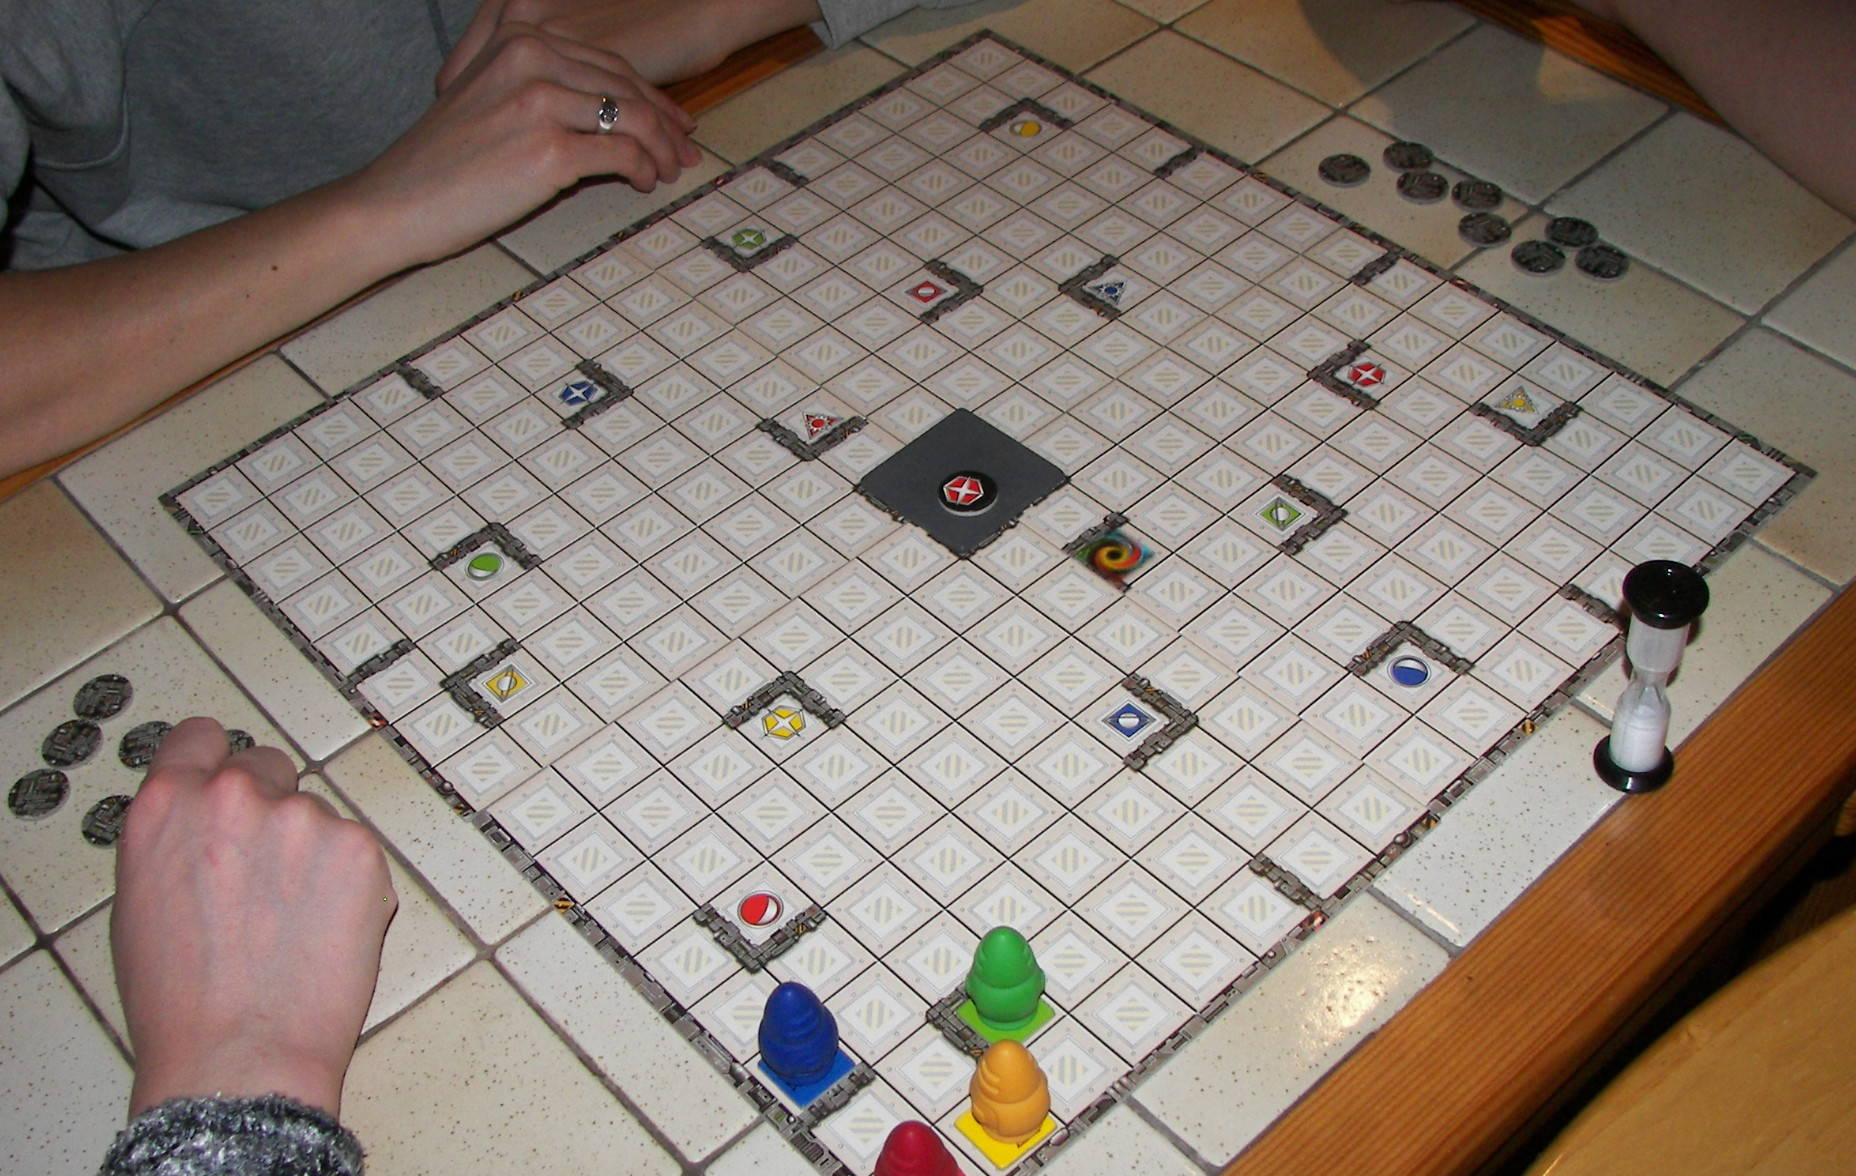
\includegraphics[scale=0.5]{images/ricochetrobot.jpg}
\end{figure}

\newpage %%%%%%%%%%%%%%%%%%%%%%%%%%%%%%%%%%%%%%%%%%%%%%%%%%%%%%%%%%%%%%%%%%%%%%%%%%%%%%%%%%%%%%%%%%%%%%%%%%%%%%%%%%%%%%%%%%%%%%%%
%table des matières

\tableofcontents

\newpage %%%%%%%%%%%%%%%%%%%%%%%%%%%%%%%%%%%%%%%%%%%%%%%%%%%%%%%%%%%%%%%%%%%%%%%%%%%%%%%%%%%%%%%%%%%%%%%%%%%%%%%%%%%%%%%%%%%%%%%%
\section{Introduction}
Le Ricochet Robots est à l'origine un jeu de plateau. D'après Wikipédia\cite{Wikipedia}, ce jeu de société est composé d'un plateau, de tuiles représentant chaque case du plateau, et de pions appelés "robots" et "jetons". Différents jetons sont imprimés dans certaines des cases (au nombre de 17). Le jeu commence en piochant un pion "jeton" parmi les 17. La case à aller correspond au symbole du jeton qui a été tiré aléatoirement. La partie est décomposée en tours de jeu, un tour consistant à déplacer les robots sur le plateau afin d'emmener le robot de la même couleur du jeton tiré sur la case correspondante. Les robots ne peuvent que se déplacer qu'en ligne droite jusqu'à rencontrer un obstacle (un robot ou un mur).

    \paragraph{}
    Le Ricochet Robot peut aussi bien être joué seul qu'avec un grand nombre de participants. Le jeton revient à la personne qui aura trouvé la séquence de mouvement qui permettra à un robot donné (parmi quatre), d'atteindre la case, en moins de coups possible dans un délai de temps imparti. La partie se termine lorsque tout les jetons auront été tirés. Le gagnant est la personne qui aura récolté le plus de jetons.
    
    \paragraph{}
    Le but de ce projet à été de développer un programme permettant de trouver une solution optimale pour toute situation du jeu. La conception de ce projet à été réalisée en plusieurs temps:
        \begin{enumerate}
            \item Le développement du moteur du jeu suivant les règles du Ricochet Robots
            \item La réalisation d'une interface graphique.
            \item L'implantation d'un algorithme de résolution naïf, appelé A*.
            \item Proposer des méthodes d'optimisation de l'algorithme, par soucis de complexité pour être résolu dans de bonnes conditions.
        \end{enumerate}

\newpage %%%%%%%%%%%%%%%%%%%%%%%%%%%%%%%%%%%%%%%%%%%%%%%%%%%%%%%%%%%%%%%%%%%%%%%%%%%%%%%%%%%%%%%%%%%%%%%%%%%%%%%%%%%%%%%%%%%%%%%%

\section{Organisation du projet}

    \subsection{Gestion du projet}

		Afin de faciliter la communication et le bon déroulement de la conception de notre jeu, divers moyens ont été mis en oeuvre.

        \subsubsection{Hébergement du code}
        
            Afin de faciliter la gestion du projet, nous avons utilisé à la fois \href{https://forge.info.unicaen.fr/}{la Forge} d’Unicaen et \href{https://github.com/}{Github} qui permettent de créer et d’administrer des dépôts sous Git très facilement par l’intermédiaire d’une interface web. D’autres fonctionnalités sont disponibles  sur ces plateformes comme une gestion des permissions, une visualisation des différents commits, la visualisation de l’activité du projet, etc. L'utilisation supplémentaire de \href{https://github.com/}{Github} permettait de centraliser les projets du cursus de la licence sur une seule plateforme ainsi que l'utilisation de "Webhooks" (envoi de notifications sur \href{https://discordapp.com/}{Discord} lors de la mise en ligne d'une fonctionnalité).
            
		\subsubsection{Gestionnaire de version}

			Nous avons utilisé un gestionnaire de version afin de permettre la centralisation du code et rendre le travail en équipe bien plus efficace. Nous avons opté pour Git, qui est un gestionnaire de version que nous avons utilisé dans un précédent projet. L'utilisation de Git rend l'utilisation des branches plus facile, permet de faire des commits sans pour autant être connecté sur le serveur. Cela permet de faire plus de commits, qui sont enregistrés localement et de les envoyer sur le serveur en une seule fois, au moment où nous sommes sûrs que la fonctionnalité ajoutée fonctionne. Git permet également de transférer facilement son code vers un autre hébergeur en ajoutant simplement une "route" (remote), tout en conservant la totalité des commits réalisés.

		\subsubsection{Trello}

			Concernant la répartition et le listage du travail à effectuer, nous avons fait le choix d'utiliser \href{https://trello.com/}{Trello}, une plate-forme qui nous permet l'utilisation de tableaux afin de planifier le projet.

			\begin{figure}[H]
				\centering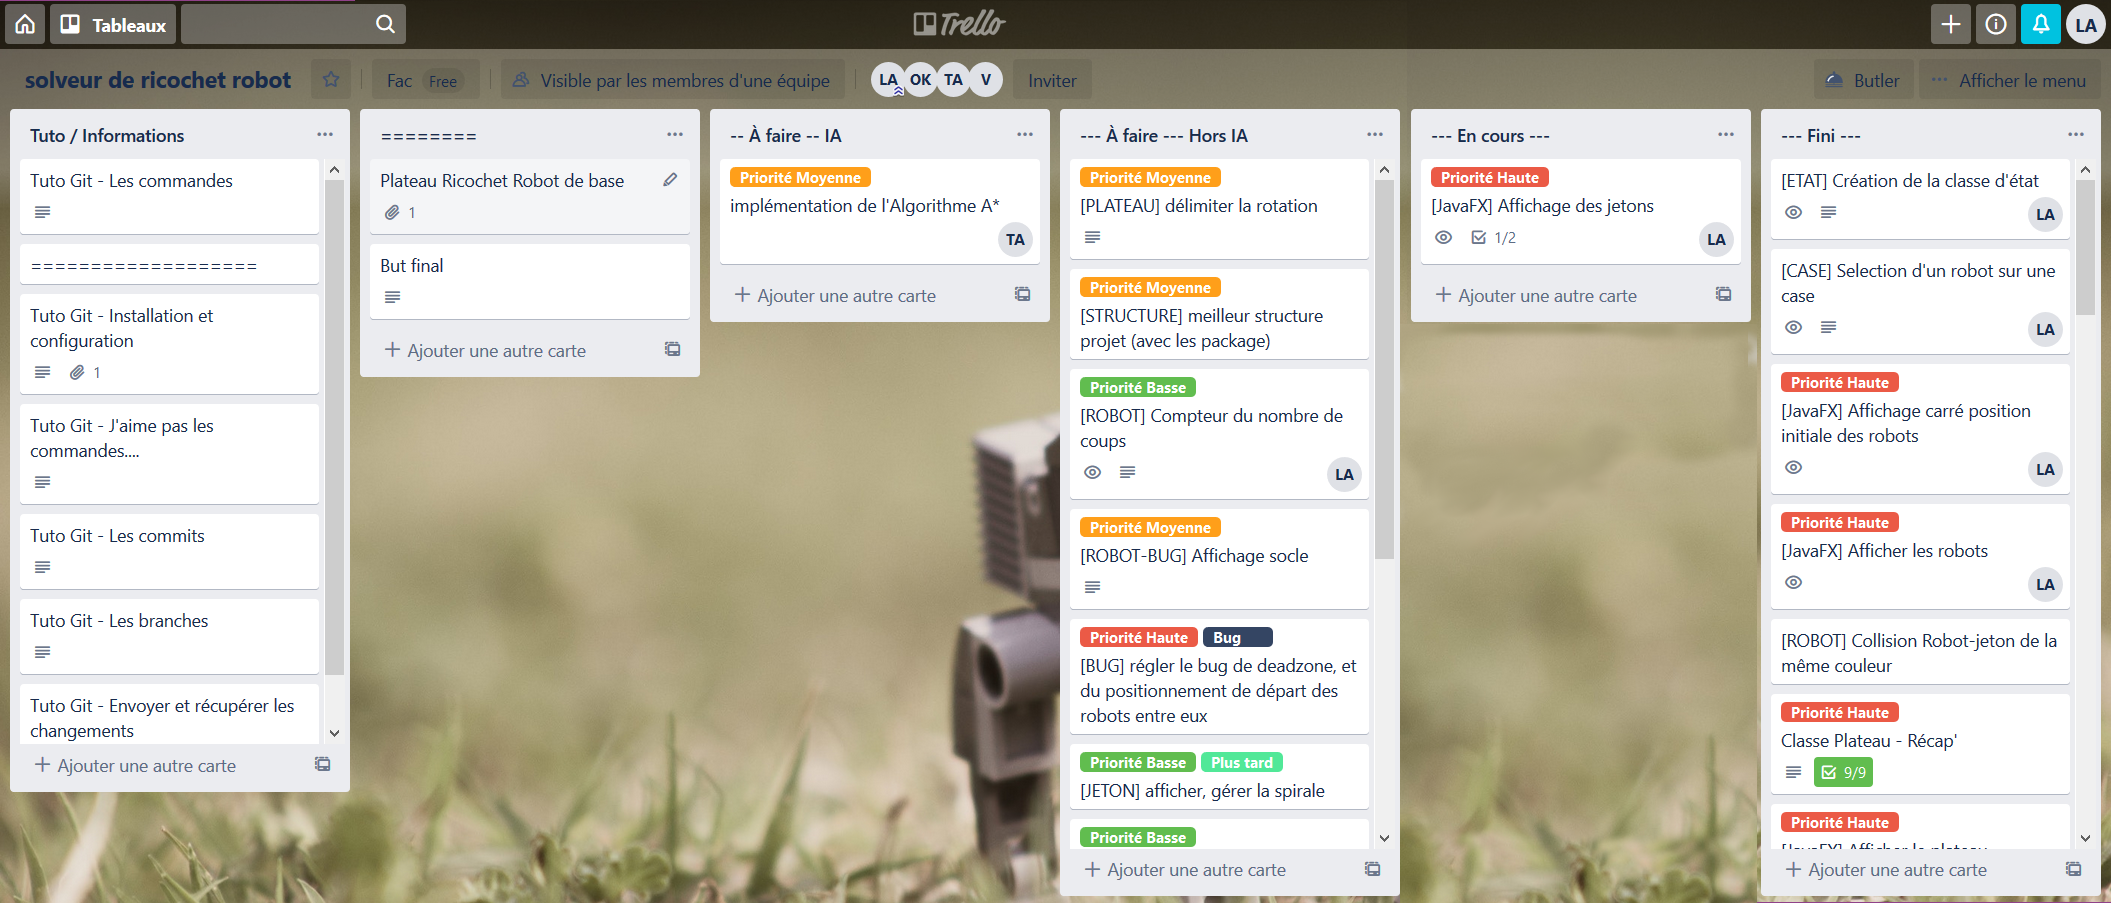
\includegraphics[width=0.95\textwidth]{images/trello.png}
				\caption{Notre tableau Trello}
			\end{figure}

			Ainsi, comme nous pouvons le constater sur l'image ci-dessus, les différentes tâches passent par différents états appelés "\textit{À faire}", "\textit{En cours}", "\textit{À modifier et à vérifier}", et "\textit{Fini}".

			La colonne "\textit{À modifier et à vérifier}" est utilisée lorsqu'une tâche est réalisée, mais doit être modifiée (car elle n'est pas optimale) ou doit être soumise à évaluation et/ou relecture. Cela permet d'éviter d'éventuels bugs par la suite mais aussi de garder une cohérence au travers du code. Lorsque cette tâche est modifiée et/ou vérifiée, elle est déplacée dans la colonne "\textit{Fini}".

		\subsubsection{Discord}

			Afin de faciliter la communication au sein du groupe, nous avons utilisé le service de messagerie \href{https://discordapp.com/}{Discord}  car tous les membres du groupe l'utilisaient déjà de manière personnelle. Ce service permet de parler par le biais de "serveurs" gratuits dans lesquels nous pouvons ajouter des salons textuels ou des salons vocaux à volonté.

			\begin{figure}[H]
				\centering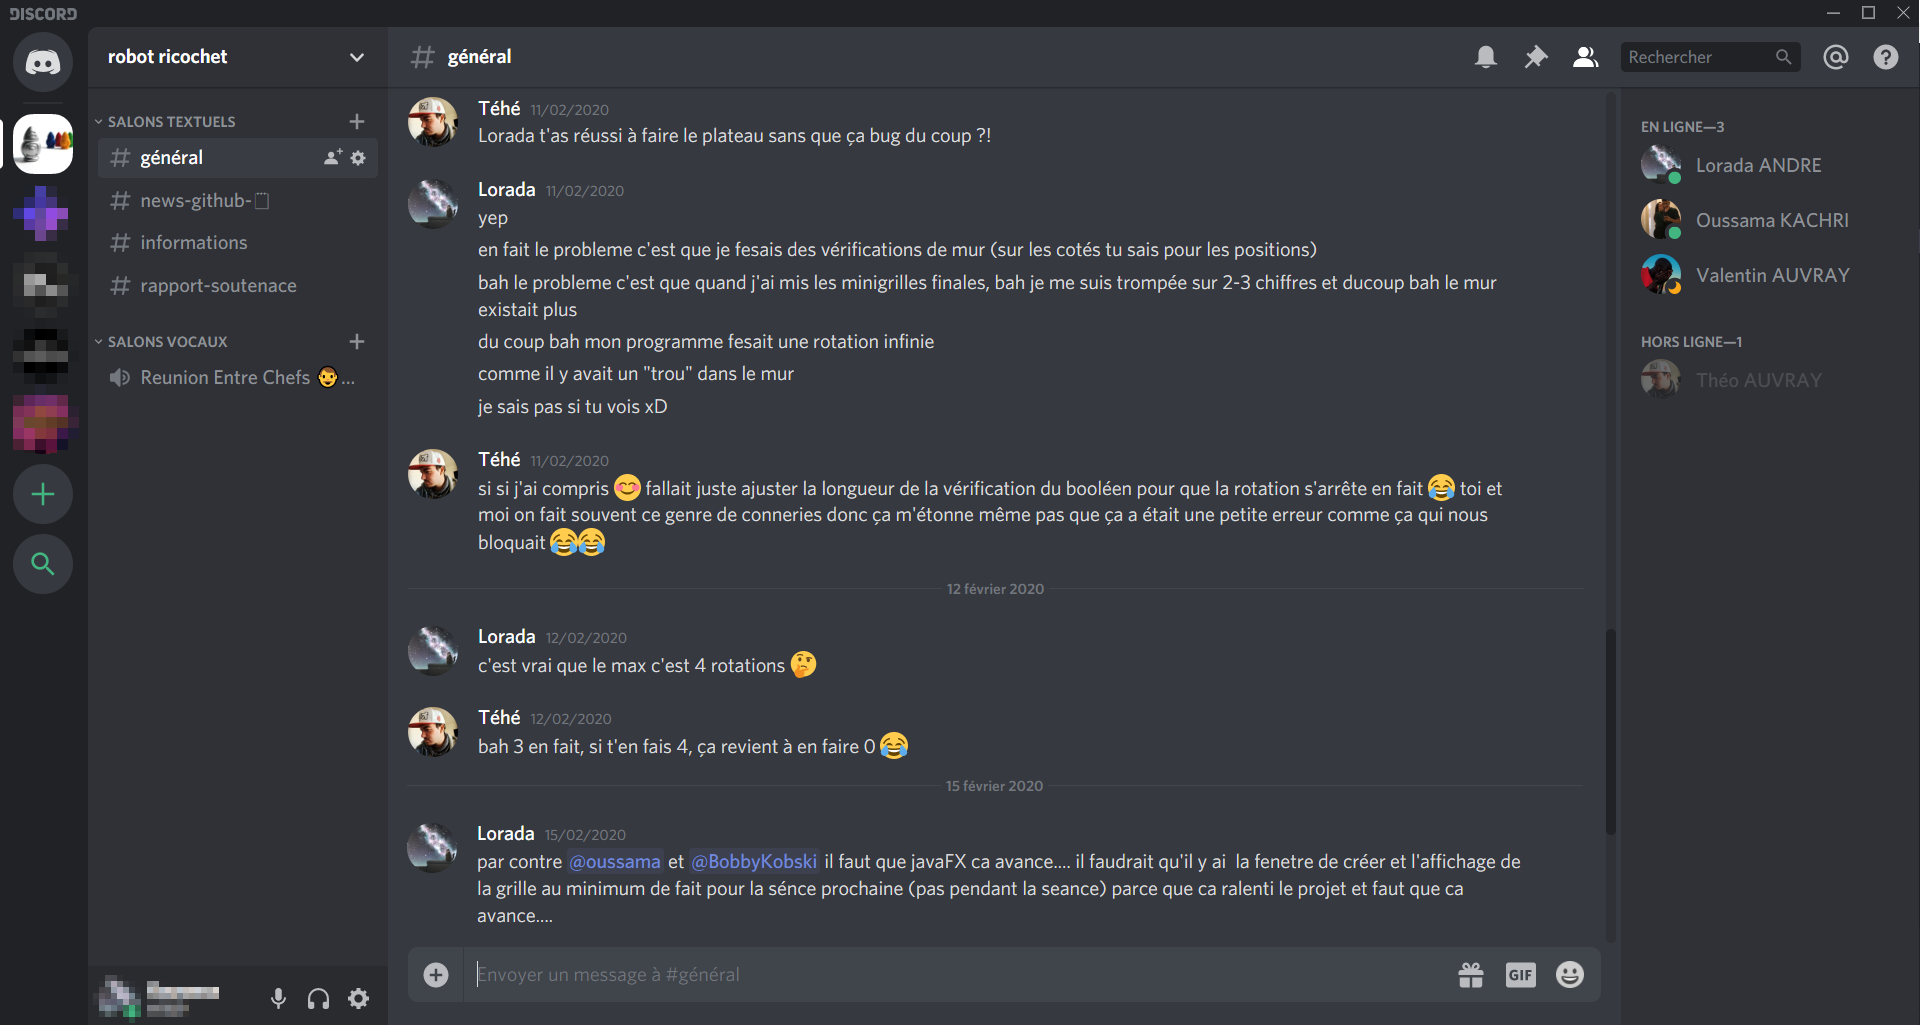
\includegraphics[scale=1]{images/discord.png}
				\caption{Notre serveur Discord}
			\end{figure}
			
			 Ainsi, nous avions un salon de discussion, nommé "\textit{informations}". Comme son nom l'indique, il permet de transmettre des messages importants sur ce qui a été fait, sur des changements importants concernant le projet, etc. Un deuxième se nommant "\textit{news-Github}" servait à recevoir une notification dès qu'une personne ajoutait du code sur \href{https://github.com/}{Github}, afin de connaître l'avancement de chaque personne sans pour autant devoir aller sur les hébergeurs, ou bien pour qu'une personne sache à quel moment elle devait reprendre le relais sur une fonctionnalité. Le troisième salon se nommant"\textit{général}" était utilisé pour les discutions beaucoup plus générales. Sur ce salon, nous pouvions discuter du projet, de certains choix à faire, ou bien demander de l'aide ou aider des membres en difficulté.
			
			
    \subsection{Répartition des tâches}
    
    \begin{center}
        \begin{tabular}{|p{7cm}|>{\centering\arraybackslash}p{4cm}|>{\centering\arraybackslash}p{4cm}|}
            \hline
                Tâches & Lorada & Théo \\
            \hline %................
                \rowcolor{ashgrey} Plateau  & &\\
                 Création de la classe Plateau & X & \\
                 \hline
                 Création des quarts de plateau & X & \\
                 \hline
                 Assemblage des quarts de plateau &  & X \\
                 \hline
                 Génération aléatoire du plateau & X & \\
                 \hline
                 Rotation des quarts de plateau & X & \\
                 \hline
                 Affichage graphique du plateau & X & \\
            \hline %................
                \rowcolor{ashgrey} Robot  & &\\
                 Création de la classe &  & X \\
                 \hline
                 Positionnement aléatoire des robots & X &\\
                 \hline
                 Collisions des robots avec les éléments & X &\\
                 \hline 
                 Déplacement des robots & X &\\
                 \hline 
                 Sélection d'un robot & X &\\
                 \hline
                 Affichage des robots et des socles & X & \\
            \hline %................
                \rowcolor{ashgrey} Jeton  & &\\
                 Création de la classe Jeton & X & \\
                \hline
                Génération aléatoire du jeton tiré & & X\\
                \hline
                Affichage graphique du jeton tiré & X & \\
             \hline %................
                \rowcolor{ashgrey} Case  & &\\
                 Création de la classe Case & X & \\
                 \hline
                 Positionnement des cases & X & \\
                  \hline
                Rotation des cases & X & \\
                \hline
                 Affichage graphique des cases & X & \\
            \hline %................
                \rowcolor{ashgrey} Case Jeton   & &\\
                Création de la classe Case Jeton & X & \\
                \hline
                Positionnement des jetons & & X\\
                \hline
                Rotation des cases jeton & X & \\
                 \hline
                Affichage graphique des cases jetons & X & \\
            \hline %................
                \rowcolor{ashgrey} Pattern Observer  & &\\
                Implémentation du pattern observer & X & \\   
            \hline %................
                \rowcolor{ashgrey} State & &\\
                 Création de la classe State & X & \\
                 \hline
                Création de l'état initial du jeu & X & \\   
                \hline
                Déplacement du robot avec le clavier & X &\\
                \hline
                Séléction du robot qui doit jouer & X &\\
                \hline
                Définition de l'état gagnant & X &\\
            \hline %................
             \rowcolor{ashgrey} Algorithme A* & &\\
                Algorithme BFS & X & \\   
                \hline
                 Sortie Anticipée & X &\\  
                \hline
                 Mise en place de l'heuristique & X &\\  
                \hline
             \hline %................
             \rowcolor{ashgrey} Documents & &\\
             Rédaction du rapport & X & \\
             \hline
             Rédaction du support de soutenance & X & \\
            \hline %................
        \end{tabular}
    \end{center}
    
\newpage %%%%%%%%%%%%%%%%%%%%%%%%%%%%%%%%%%%%%%%%%%%%%%%%%%%%%%%%%%%%%%%%%%%%%%%%%%%%%%%%%%%%%%%%%%%%%%%%%%%%%%%%%%%%%%%%%%%%%%%%

\section{Architecture du projet}
    \subsection{Arborescence du projet}
    
        Le projet est structuré de la manière suivante:
        
        \begin{figure}[H]
    		\centering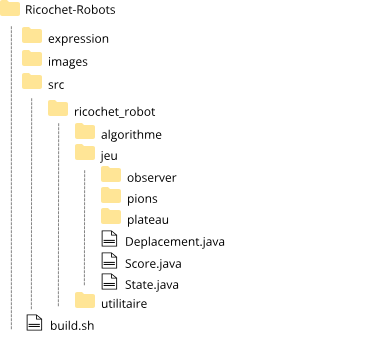
\includegraphics[width=0.5\textwidth]{images/dossier.png}
    		\caption{Arborescence du projet}
    	\end{figure}
    	
    	\paragraph{}
    	Á la racine de ce projet, nous y retrouvons:
    	
    	\begin{description}
    	    \item [expression:] contient ce rapport et le diaporama pour la soutenance.
    	    \item [images:] contient l'ensemble des images utilisées pour la partie interface graphique du jeu.
    	    \item [src:] contient le code source du projet.
    	    \item [build.sh:] le script de compilation du projet.
    	\end{description}
    	
    \subsection{Architecture du programme}
    
        \subsubsection{Diagramme des packages}
            
            \paragraph{}
             Le code source est organisé dans différents packages:
             
            \begin{description}
            \item[algorithme:] contient les classes relatives à l'implémentation de l'algorithme A*.
                 \item[jeu:] contient tout les éléments relatifs au jeu.
                 \begin{description}
            	    \item[observer:] regroupe les différentes classes utilisées pour l'implémentation du pattern observer.
            	    \item[pions:] contient les classes représentants les éléments mobiles du Ricochet Robots, correspondant aux robots et aux jetons du jeu.  
            	    \item[plateau:] contient les classes relatives à la création du plateau
        	    \end{description}
                 \item[utilitaire:] contient une classe utilitaire.
             \end{description}
             
            \begin{figure}[H]
                \centering
                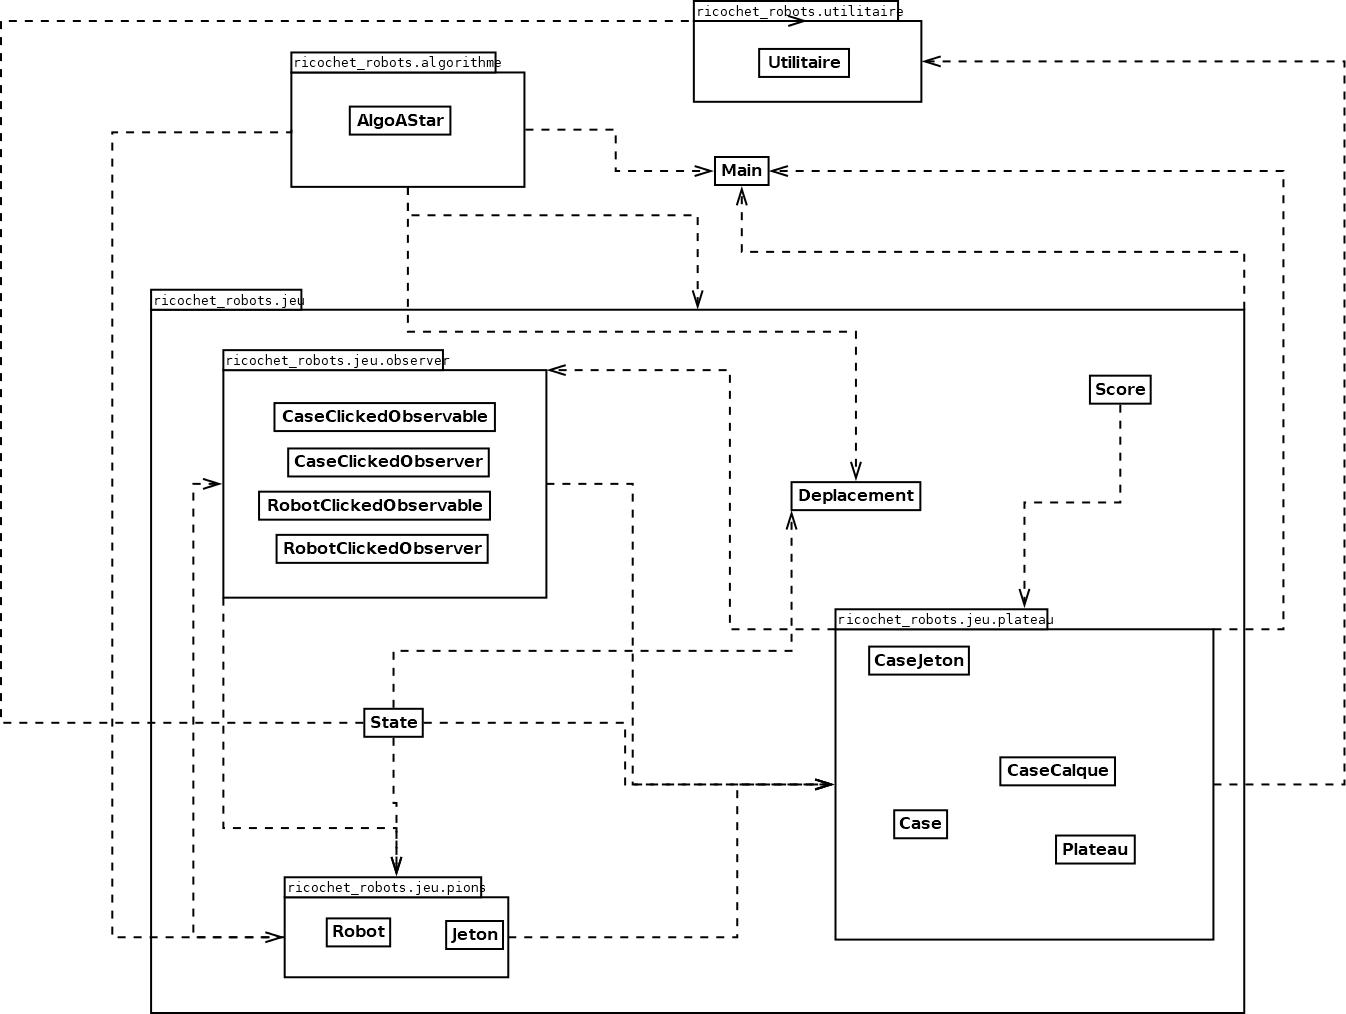
\includegraphics[scale=0.3]{images/diagrammePackage.png}
                 \caption{Diagramme des packages}
            \end{figure}

            \newpage
            
        \subsubsection{Diagramme des classes}
        
            \begin{figure}[H]
                \centering
                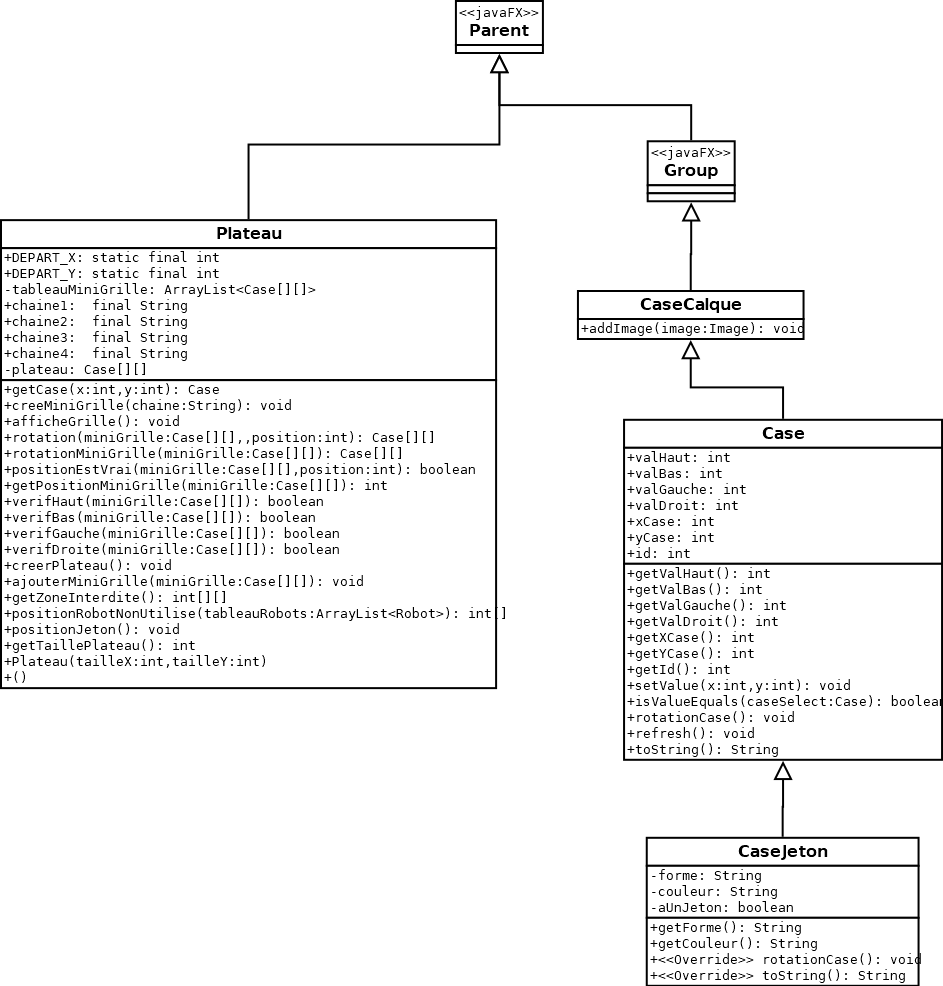
\includegraphics[scale=0.45]{images/diagrammePlateau.png}
                \caption{Diagramme du package plateau}
            \end{figure}
            
            
 %%%%%%%%%%%%%%%%%%%%%%%%%%%%%%%%%%%%%%%%%%%%%%%%%%%%%%%%%%%%%%%%%%%%%%%%%%%%%%%%%%%%%%%%%%%%%%%%%%%%%%%%%%%%%%%%%%%%%%%%

\section{Développement du jeu}
    \subsection{Création du plateau}
        \subsubsection{Création des mini-plateaux}
            Pour concevoir le Ricochet Robot, la première question que nous nous sommes posé à été: "comment devons-nous créer le plateau?". Le plateau du Ricochet Robots est un ensemble de "mini-plateaux" qui, une fois assemblés, forment ce plateau. Dans la version du jeu de société, il existe quatre morceaux de plateaux, chaque morceau ayant deux faces. Dans notre version, nous avons voulu garder que quatre faces, une pour chaque morceau, qui étaient suffisantes pour la réalisation du Ricochet Robot.
            
            \begin{figure}[H]
            	\centering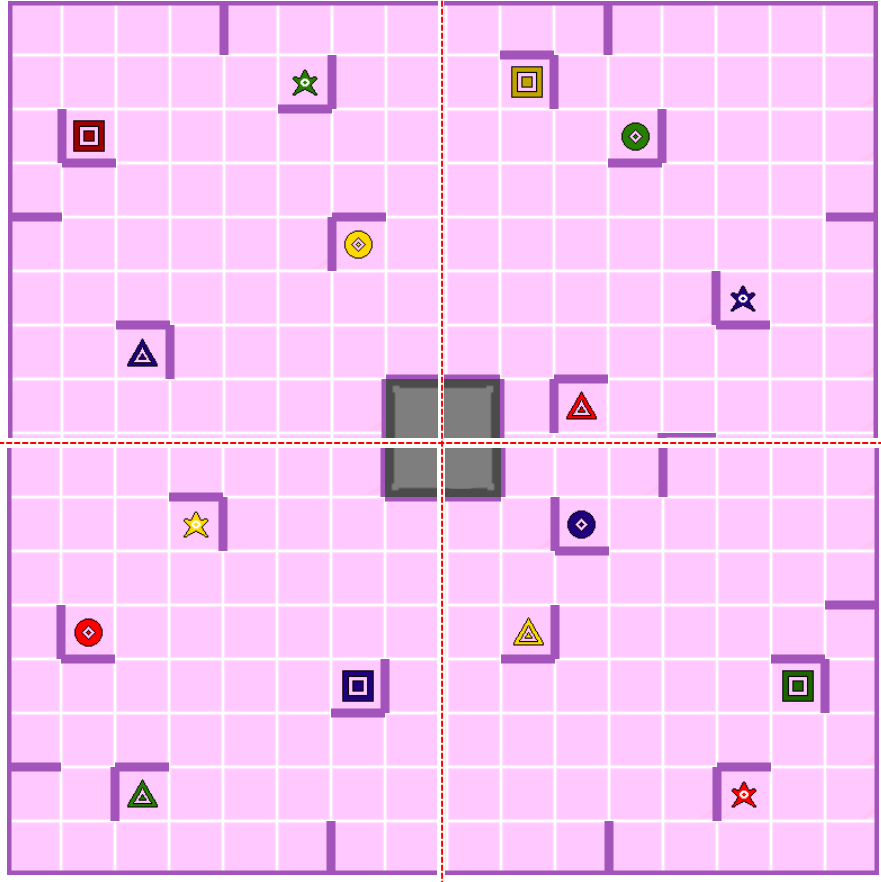
\includegraphics[width=0.5\textwidth]{images/plateauDecoupe.png}
            	\caption{Composition du plateau}
            \end{figure}
            
            Pour créer le plateau, nous devions commencer par la création de ces mini-plateaux. Ces quatre mini-plateaux sont chacun représenté sous forme de tableaux à deux dimensions, contenant des cases et des murs. 
            
            C'est à ce moment là que nous avions réfléchi sur la représentation de ces cases et de ces murs. Après observation du plateau, nous avions remarqué que ce plateau était composé que de onze cases différentes.
            
            \begin{figure}[H]
            	\centering
\includegraphics[scale=0.60]{images/liste_cases.png}
            	\caption{Ensemble des cases existantes}
            \end{figure}
            
            Ces cases ont toutes un élément en commun: la possibilité d'avoir un mur en haut, en bas, à gauche, ou à droite.
    
            \vspace{0.5cm}
            \begin{center}
                \begin{tikzpicture}
                    \draw (1,1) rectangle (5,5);
                    \draw[color=red] (1,1.5) -- (5,1.5);
                    \draw[color=green] (1,4.5) -- (5,4.5);
                    \draw[color=blue] (1.5,1) -- (1.5,5);
                    \draw[color=olive] (4.5,5) -- (4.5,1);
                    \node[color=red] (pos) at (3,0.5) {BAS};
                    \node[color=green] (pos) at (3,5.5) {HAUT};
                    \node[color=blue] (pos) at (0,3) {DROIT};
                    \node[color=olive] (pos) at (6,3) {GAUCHE};
                    
                    \node (posi) at (10,5) {[ HAUT, DROIT, BAS, GAUCHE ]};
                    \draw[->] (5,4) -- (posi);
                \end{tikzpicture}
            \end{center}  
            \vspace{0.5cm}
            
            Nous avons donc décidé de représenter chaque case de cette manière: la présence d'un mur en haut entraînait un 1 à la valeur de HAUT, la présence d'un mur à droite entraînait un 1 à la valeur de DROIT, et ainsi de suite pour les autres côtés. Ce qui donne par exemple:
            
            \vspace{0.5cm}
            
            \begin{figure}[H]
                \centering
                \begin{tikzpicture}
                    \draw[fill=red] (0,2) rectangle (2, 1.75);
                    \draw (0,0) rectangle (2,2);
                    \draw[dotted] (0,0.25) -- (2,0.25);
                    \draw[dotted] (0,1.75) -- (2,1.75);
                    \draw[dotted] (0.25,0) -- (0.25,2);
                    \draw[dotted] (1.75,0) -- (1.75,2);
                    
                    \node (bool) at (6,1) {[ True, False, False, False ]};
                    \node (bin) at (10,1) {[1,0,0,0]};
                    \draw[->] (bool) -- (bin);
                \end{tikzpicture}
                \caption{Cas de figure pour un mur en haut de la case}
            \end{figure}
            
    
            Pour ne pas alourdir chaque mini-plateau en créant pour chacun d'entre eux un tableau à trois dimension (un tableau en deux dimensions dont chaque élément contient elle-même un tableau), nous avons donc créé une classe Case, contenant les quatre variables précédemment évoquées, nommées "valHaut, valBas, valGauche et valDroite" qui remplacent le format de tableau [HAUT, DROIT, BAS, GAUCHE]. Nous obtenons alors avec un tableau à deux dimension dont chaque élément contient une instance de Case.
            
            Á ce moment là, c'était au tour de la création des quatre mini-tableaux. La position de chaque case de chaque mini-tableau est importante et inchangeable, car les modèles des mini-plateaux du jeu de société sont réalisés de manière à avoir une solution à toute situation de jeu. Nous avons donc gardé les modèles existants. 
            
            Nous avons donc cherché une manière de sauvegarder ces quatre modèles de mini-plateau dans le code, et ainsi qu'à partir de cette sauvegarde, les mini-plateaux se créent. 
            
            Nous avons opté pour un modèle suivant:
            \vspace{0.5cm}
            \lstinputlisting[language=Java]{code/var.java}
    
            
            Cette manière de faire permettait qu'à partir d'une suite de nombres, le programme créé un mini-plateau. Le code correspondant est le suivant:
                
            \begin{algorithm}[H]%-------------------------------------------
                \DontPrintSemicolon
                \KwIn{Une chaine de caractère représentant le mini-plateau}
                \KwOut{Le mini-plateau}
                $tableauDeChiffre \gets chaineDeCaractere.split(",")$
                $tailleTableau \gets \sqrt{tableauDeChiffre.length()}$
                $index \gets 0$
                $miniGrille[][] \gets {nouvelle \ instance \ de \ Case }$
                \For{$y \gets 0$ \textbf{à} $tailleTableau$}{
                  \For{$x \gets 0$ \textbf{à} $tailleTableau$}{
                    $miniGrille[x][y] \gets new \ Case(Utilitaire.intToBinary(tab1D[index]), x, y)$
                    $index++$
                    }
                 }
                \Return{$miniGrille$}\;
                \caption{\sc Création d'un mini-plateau}
            \end{algorithm}%-------------------------------------------
            
            Chaque nombre correspond à un identifiant d'une case. Le numéro n'est pas pris au hasard: en reprenant la figure 8 ci-dessus, nous avons vu que une case ayant un mur en haut correspondait à [1,0,0,0]. L'idée était de récupérer ces chiffres, formant "1000", qui en nombre binaire donne un "8". Une case avec un mur en haut correspond donc au chiffre "8". Le système est le même pour chaque case.
            
            \subsubsection{Positionnement des mini-plateaux}
    
            Comme le plateau est composé de quatre parties, chaque mini-plateau ont quatre possibilités de positionnement afin de former le plateau final (plus exactement: 4 - le nombre de mini-plateau déjà positionné).
        
            \begin{center}
                \begin{tikzpicture}
                    \draw (0,0) rectangle (4,4);
                    \draw[dotted] (0,2) -- (4,2);
                    \draw[dotted] (2,0) -- (2,4);
                    \node (4) at (1,1) {4};
                    \node (3) at (3,1) {3};
                    \node (2) at (3,3) {2};
                    \node (1) at (1,3) {1};
                \end{tikzpicture}
            \end{center}
            
            Pour les positionner de manière aléatoire, nous avons fait en sorte que le programme tire une position pour chaque mini-plateau. Cependant ce n'est pas suffisant, puisqu'il fallait que les murs de chaque mini-plateau soient bien positionnés, sinon nous nous retrouverions avec des "mauvais plateaux" de cette forme:
            
            \begin{figure}[H]
                \centering
                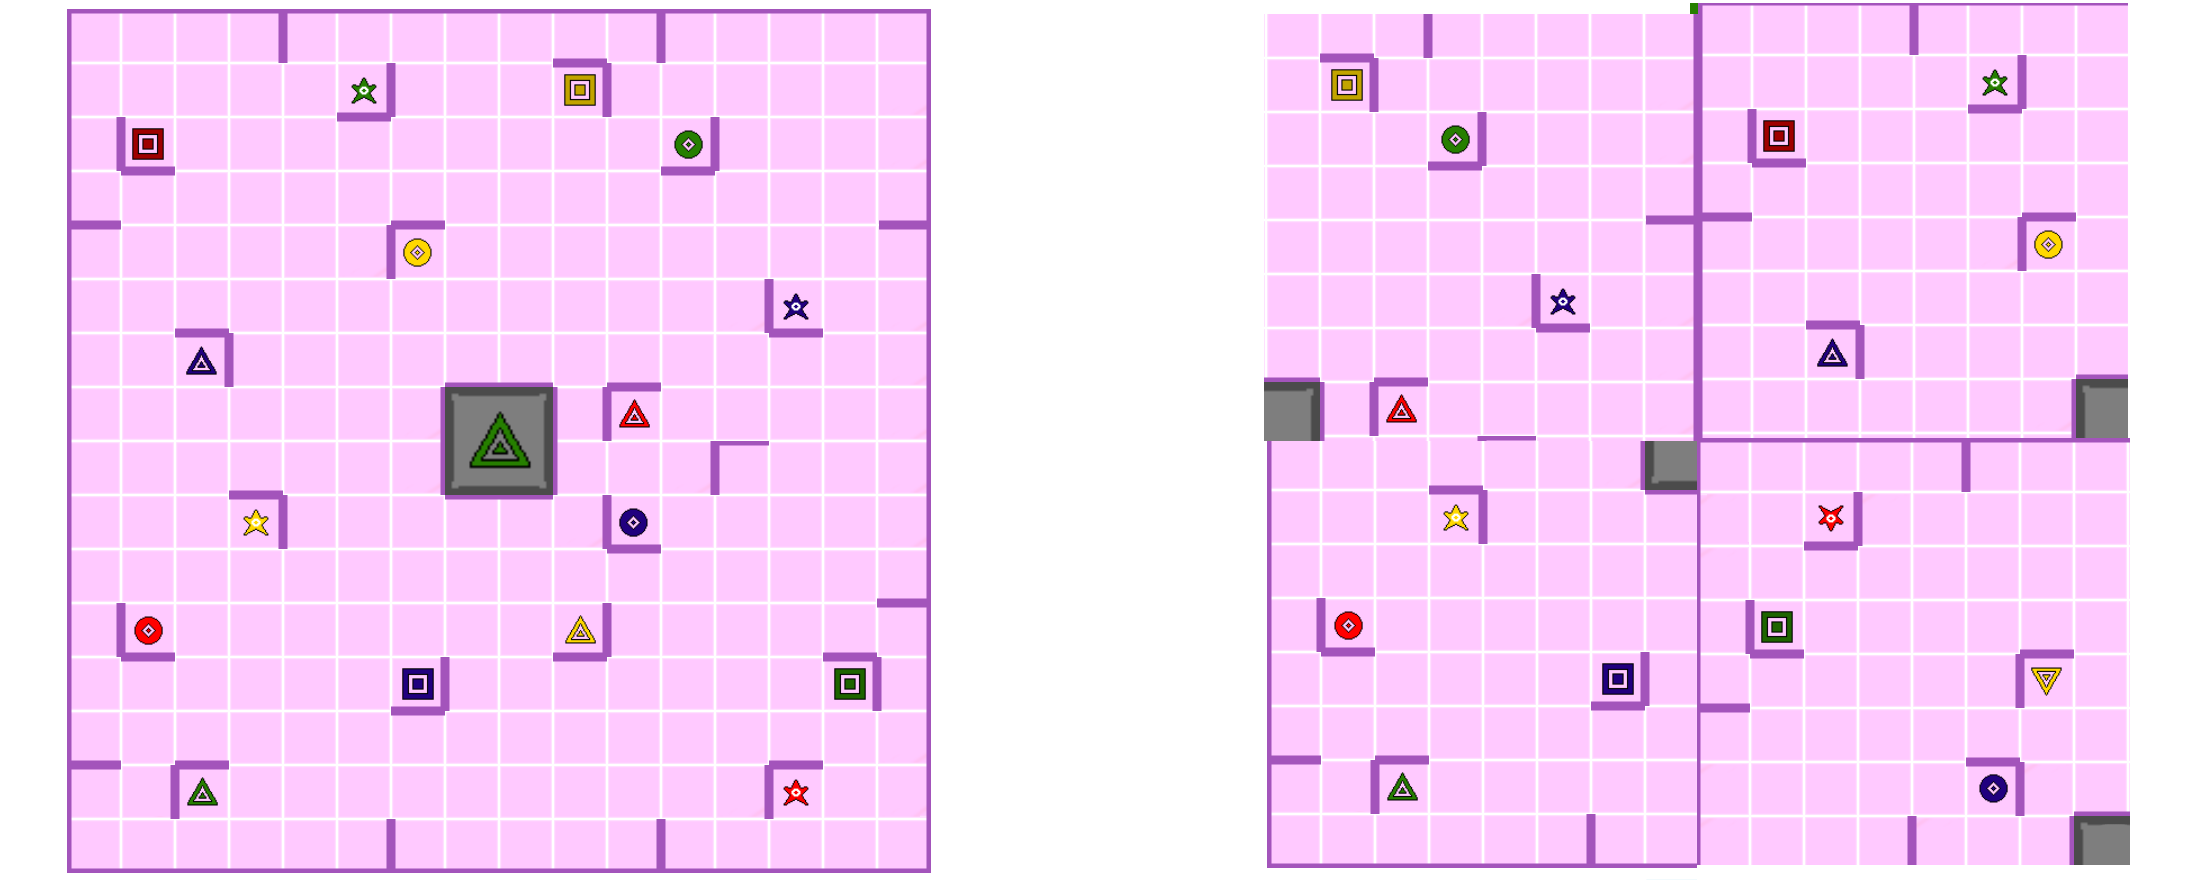
\includegraphics[scale=0.2]{images/bonvsmauvais.png}
                \caption{Bon (à gauche) et mauvais plateau (à droite)}
            \end{figure}
            
            
            Pour cela, il fallait vérifier l'emplacement des murs qui composent les bordures, et affecter une rotation à ces mini-plateaux tant que le mini-plateau n'est pas valide par rapport à sa position affectée. Les algorithmes qui représentent ce dispositif sont les suivants:
            
            \newpage
            
            \begin{algorithm}[H]%-------------------------------------------
                \DontPrintSemicolon
                \KwIn{le mini-plateau, la position affectée au mini-plateau}
                \KwOut{Le mini-plateau}
                $miniGrilleRota \gets new \ Case(miniGrille.length(), miniGrille.length())$
                
                \For{$y \gets 0$ \textbf{à} $miniGrille.length()$}{
                  \For{$x \gets 0$ \textbf{à} $miniGrille.length()$}{
                        $miniGrilleRota[x][y] \gets miniGrilleRota[x][y]$
                    }
                 }
                 \While{positionEstVraie(miniGrilleRota, position) != true}{
                    $miniGrilleRota[x][y] \gets rotationMiniGrille(miniGrilleRota)$
                 }
                \Return{$miniGrilleRota$}\;
                \caption{\sc Rotation d'un mini-plateau}
                Avec positionEstVrai(), une méthode qui permet de vérifier les murs des bordures
            \end{algorithm}%-------------------------------------------
        
            \begin{algorithm}[H]%-------------------------------------------
                \DontPrintSemicolon
                % \SetKwData{JeuNonTrie}{jeuNonTrie}
                % \SetKwData{JeuTrie}{jeuTrie}
                \KwIn{un mini-plateau}
                \KwOut{Le mini-plateau dans une rotation de 90 degrés}
                $miniGrilleRota \gets new \ Case(miniGrille.length(), miniGrille.length())$
                
                \For{$y \gets 0$ \textbf{à} $miniGrille.length()$}{
                  \For{$x \gets 0$ \textbf{à} $miniGrille.length()$}{
                        $miniGrilleRota[x][y] \gets miniGrilleRota[y][miniGrille.length - x - 1]$
                        $miniGrilleRota[x][y].rotationCase()$
                    }
                 }
                 \While{positionEstVraie(miniGrilleRota, position) != true}{
                    $miniGrilleRota[x][y] \gets rotationMiniGrille(miniGrilleRota)$
                 }
                \Return{$miniGrilleRota$}\;
                \caption{\sc Rotation du mini-plateu de 90 degrés}
            \end{algorithm}%-------------------------------------------
            
            \vspace{0.8cm}
            La méthode rotationCase consiste à décaler d'un cran les valeurs de la classe Case selon le modèle suivant:
            
           \begin{figure}[H]
               \centering
               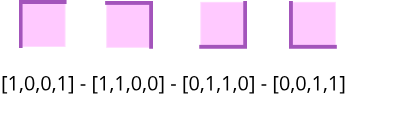
\includegraphics[scale=0.7]{images/rotaCase.png}
           \end{figure}
           
           Le code est le suivant:
           
            \lstinputlisting[language=Java]{code/rotaCase.java}
            
        La méthode caseToInt permet de recalculer l'identifiant de la case, qui aura changé après la rotation d'une case.
            
                
        \subsubsection{Création du plateau}
            Une fois que chaque mini-plateau se trouvait dans la bonne rotation correspondant à sa position, c'est à ce moment là que nous devions créer le plateau, en assemblant ces mini-plateaux entre eux. Pour cela, nous avons crée un tableau à deux dimensions de type Case, représentant le plateau et chaque coin de ce plateau est parcouru pour y affecter les valeurs contenues dans chaque mini-plateau. L'algorithme utilisé est le suivant:
            
            
            \begin{algorithm}[H]%-------------------------------------------
                \DontPrintSemicolon
                \KwIn{Le mini-plateau à placer}
                $ plateau[][] \gets nouvelle \ instance \ de \ Case $
                $ demiTabX \gets divise \ le \ tableau \ en \ largeur \ par \ 2$
	        	$ demiTabY \gets divise \ le \ tableau \ en \ hauteur \ par \ 2$
                
                \If{la position du mini-plateau doit être à 1}{
                    \For{$y \gets 0$ \textbf{à} $demiTabY$}{
                        \For{$x \gets 0$ \textbf{à} $demiTabX$}{
                            $plateau[x][y] \gets miniPlateau[x][y]$
                        }
                    }
                }
                \uElseIf{la position du mini-plateau doit être à 2}{
                    \For{$y \gets 0$ \textbf{à} $demiTabY$}{
                        \For{$x \gets demiTabX$ \textbf{à} $tableau.length$}{
                            $plateau[x][y] \gets miniPlateau[x-demiTabX][y]$
                        }
                    }
                }
                \uElseIf{la position du mini-plateau doit être à 3}{
                    \For{$y \gets demiTabY$ \textbf{à} $tableau.length$}{
                        \For{$x \gets demiTabX$ \textbf{à} $tableau.length$}{
                            $plateau[x][y] \gets miniPlateau[x-demiTabX][y-demiTabY]$
                        }
                    }
                }
                \uElseIf{la position du mini-plateau doit être à 4}{
                    \For{$y \gets demiTabY$ \textbf{à} $tableau.length$}{
                        \For{$x \gets 0$ \textbf{à} $demiTabX$}{
                            $plateau[x][y] \gets miniPlateau[x][y-demiTabX]$
                        }
                    }
                }
                
                \caption{\sc Création du plateau}
            \end{algorithm}%-------------------------------------------
    \newpage
    \subsection{Positionnement des robots}
        Lors du lancement du jeu, les robots ne pouvaient pas être positionnés sur n'importe quelle case. Certaines cases étaient dites "interdites". Il s'agissait des cases à jetons (en rouge sur l'image ci-dessous), ainsi que le centre du plateau (en jaune sur l'image ci-dessous), comme montré ci-dessous:
        
        \begin{figure}[H]
            \centering
            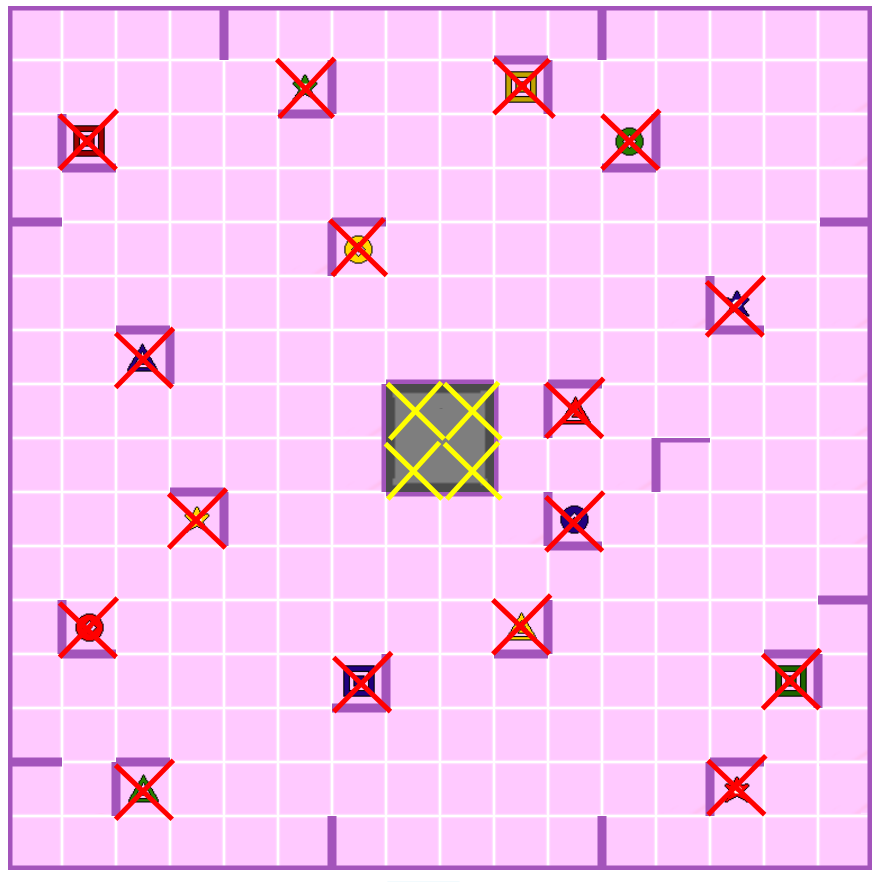
\includegraphics[scale=0.17]{images/positionInterdite.png}
            \caption{Positions initiales interdites au lancement du jeu pour les robots}
        \end{figure}
        
        Bien évidement, deux robots ne pouvaient pas se situer sur la même case. Il fallait donc également vérifier qu'à chaque nouveau robot créé, les cases utilisées par les autres robots, ne soient plus disponibles pour ce nouveau robot.
        
        Étant donné que les positions interdites étaient qu'une minorité, il était plus judicieux de d'abord tirer une position de manière aléatoire, c'est-à-dire un nombre représentant la position en abscisse du robot, et un autre pour la position en ordonnée. Á partir de ces deux nombres, il fallait ensuite vérifier si la coordonnée correspondante n'était pas similaire à une case interdite ou une position précédemment donnée à un robot. Si les coordonnées étaient correctes, alors on appliquer au robot ces coordonnées, et dans le cas où la coordonné tirée n'était pas valide, le processus recommençait tant que celles-ci n'étaient pas satisfaisantes. 
        
        L'algorithme correspondant à l'affectation des positions pour les robots est la suivante:
    
    
        \begin{algorithm}[H]%-------------------------------------------
            \DontPrintSemicolon
            \KwOut{Les coordonnées correctes pour le robot}
            $surJeton \gets false$
            $surRobot \gets false$
            $surCaseInterdite \gets false$
            
            \Do{$surJeton \ \textsc{or} \ surCaseInterdite \ \textsc{or} \ surRobot$}{
                $aleaX \gets tirage \ d'un \  nombre \  aleatoire \  entre \  0 \  et \  15$
                $aleaY \gets tirage \ d'un \  nombre \  aleatoire \  entre \  0 \  et \  15$
                \If{surJeton}{
                    $continue$
                }
                $surCaseInterdite \gets estSurCaseInterdite()$
                \If{$surCaseInterdite$}{
				    $continue$
			    }
    			\If{$robotsExistants! \gets \emptyset$}{
    				$surRobot \gets estSurAutresRobots(aleaX,aleaY)$
    
    				\If{$surRobot$}{
    					$continue$
    				}
                }
                $position[] \gets {aleaX, aleaY}$
            }
            \Return{$position[]$}
            \caption{\sc Positionnement des robots à l'état initial}
        \end{algorithm}%-------------------------------------------
        
    \subsection{Déplacements et collisions des robots}
    
        Lorsque l'on veut déplacer un robot vers une direction, le déplacement devait s'effectuer qu'en ligne droite jusqu'à ce qu'il rencontre un obstacle. L'obstacle peut être un mur ou bien un autre robot. Pour que le robot s'arrête à un obstacle, il fallait mettre en place un système de collision. 
        
        
         \begin{figure}[H]
            \centering
            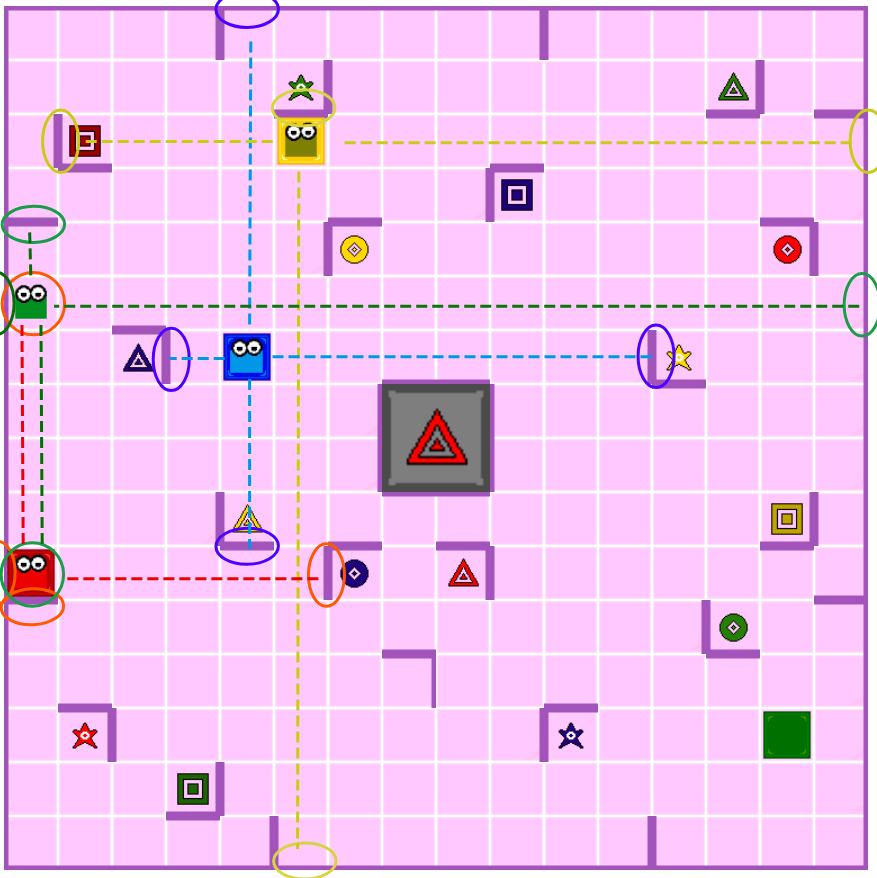
\includegraphics[scale=0.25]{images/collision.png}
            \caption{Ensemble de collisions pour chaque déplacement des robots à un état donné}
        \end{figure}
        
        Pour pouvoir mettre en place ce système de collision lors d'un déplacement, il a donc fallu faire en sorte de vérifier la case actuelle du robot à déplacer, si elle contenait un mur sur son chemin et si la case suivante contenait un mur sur son chemin ou un autre robot.
        
        \begin{figure}[H]
            \centering
            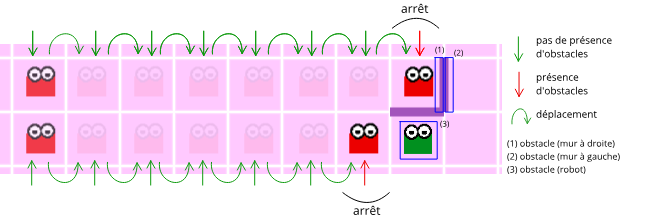
\includegraphics[scale=0.7]{images/deplacements.png}
            \caption{Vérifications lors d'un déplacement d'un robot (vers la droite sur cette image)}
        \end{figure}
        
        \l'algorithme correspondant à ces vérification est le suivant:
        
        \begin{algorithm}[H]%-------------------------------------------
            \DontPrintSemicolon
            \KwIn{La direction de déplacement}
    		\If{$direction == haut$}{
    			\While{$pas\ de \ mur\ en\ haut\ de\ la\ case\ actuelle$ \textbf{et} $pas\ de\ 
    			mur\ en\ bas de\ la\ case\ suivante $ \textbf{et}  $  !estUneCollisionRobot(direction, robot)$}{
    				$deplacement\ d'une\ case\ vers\ le\ haut$
    			}
    		}
    		\uElseIf{$direction == bas$}{
    			
    			\While{$pas\ de \ mur\ en\ bas\ de\ la\ case\ actuelle$ \textbf{et} $pas\ de\ 
    			mur\ en\ haut\ de\ la\ case\ suivante $ \textbf{et}  $  !estUneCollisionRobot(direction, robot)$}{
    				$deplacement\ d'une\ case\ vers\ le\ bas$
    			}
    		}
    		\uElseIf{$direction == gauche$}{
    			\While{$pas\ de \ mur\ a\ gauche\ de\ la\ case\ actuelle$ \textbf{et} $pas\ de\ 
    			mur\ a\ droite\ de\ la\ case\ suivante $ \textbf{et}  $  !estUneCollisionRobot(direction, robot)$}{
    				$deplacement\ d'une\ case\ vers\ la\ gauche$
    			}
    		}
    		\uElseIf{$direction == droite$}{
    			 \While{$pas\ de \ mur\ a\ droite\ de\ la\ case\ actuelle$ \textbf{et} $pas\ de\ 
    			mur\ a\ gauche\ de\ la\ case\ suivante $ \textbf{et}  $  !estUneCollisionRobot(direction, robot)$}{
    				$deplacement\ d'une\ case\ vers\ la\ droite$
    			}
    		}
            \caption{\sc Déplacement d'un robot jusqu'à collision}
        \end{algorithm}%-------------------------------------------
     
    \subsection{Sélection des robots}
        %****************** selection robots **************************%
       
        
            Pendant une partie, il est souvent nécessaire de déplacer les autres robots afin qu'ils fassent office d'obstacles, ce qui peut permettre au robot devant jouer (celui qui doit aller sur la case d'objectif) de récupérer le jeton en réalisant moins de mouvements qu'en temps normal.
            \paragraph{}
            Pour cela, nous voulions faire en sorte qu'au moment où le joueur clique sur un autre robot, c'est ce nouveau robot qui à la possibilité de se déplacer, et si le joueur clique ailleurs sur le plateau (en l'occurrence sur une case du plateau), ou sur le robot qui doit attraper le jeton, c'est de nouveau le robot devant jouer qui a la possibilité de se déplacer.
            \paragraph{}
            Pour mettre en place ce système, nous avons donc mis en place le design pattern \textit{Observer}. Ce design pattern permet dans notre projet de gérer des événements de la souris sur un robot et une case. Dans notre projet, nous avons la classe State qui est à la fois l'observeur de l'événement sur un robot et l'observeur de l'événement sur une case. D'un autre côté, du côté des observables, nous avons la classe Case (qui signale un clic sur les cases) et la classe Robot (qui signale un clic sur les robots). Le pattern observer est mis en place de la manière suivante:
            
           \begin{figure}[H]
                \centering
                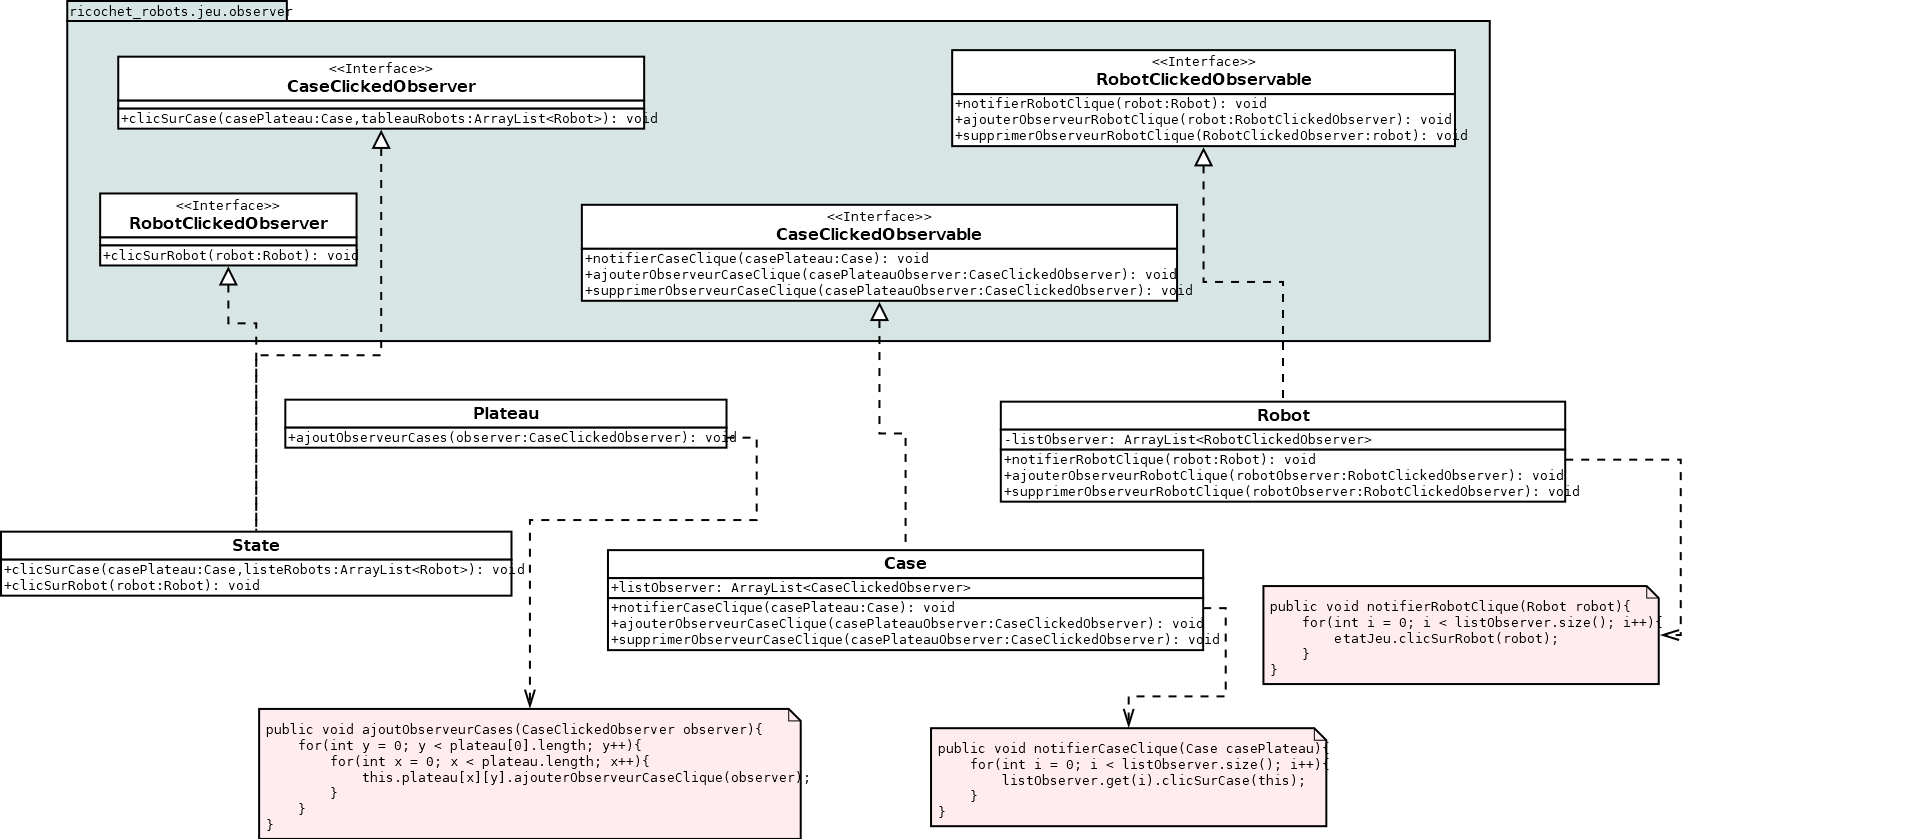
\includegraphics[scale=0.3]{images/patternObserverRobot.png}
                \caption{Diagramme de l'implémentation du pattern Observer}
            \end{figure}
            
            Lors de la création de chaque robot, nous ajoutons à chacun d'entre eux, la classe State comme observeur. Dans la classe Plateau, nous réalisons la même chose sur chacune des cases (en ajoutant la classe State comme observer). La classe State implémente les interfaces CaseClickedObserveret RobotClickedObserver. Nous retrouvons dans cette classe les méthodes à redéfinir de ces interfaces, c'est-à-dire la méthode \textit{clicSurCase(Case case)} et la méthode \textit{clicSurRobot(Robot robot)}. Cet deux méthodes contiennent l'action réalisée lors du clic sur l'un de ces objets. Dans les classes Robot et Classe, nous avons une méthode qui est redéfini des interfaces RobotClickedObservable (pour la classe Robot) et CaseClickedObservable  (pour la classe Case). Ces méthodes sont appelées lorsque le robot (ou la case) est cliqué(e). Cela permet de prévenir les observeurs du clic réalisé sur l'objet (en l'occurrence ici il s'agit uniquement de la classe State). Plus précisément, la méthode notifierRobotClique appelle directement la méthode \textit{clicSurRobot()} pusqu'elle à accès à la classe State, et la méthode \textit{notifierCaseClique()} récupère dans son ArrayList d'observeurs, les différents observeurs et appelle la méthode \textit{clicSurCase()} de chaque observateur (la classe State).
            
            Le contenu de la méthode \textit{clicSurRobot()} est le suivant: 
            \lstinputlisting[language=Java]{code/clicRobot.java}
            Cela permet de changer la valeur de la variable robotActuel, puisque le robot qui se déplace est celui qui est sauvegardé dans la variable robotActuel. Ceci permet donc de changer de robot à déplacer. 
            
            Le contenu de la méthode \textit{clicSurCase()} est le suivant:
            \lstinputlisting[language=Java]{code/clicCase.java}
            Cet appel à la méthode \textit{robotAJouer()} permet de rechercher le robot qui doit atteindre l'objectif parmi tout les robots existants. Une fois le robot trouvé, ce robot est affecté à la variable robotActuel, ce qui permet de récupérer le contrôle du robot devant jouer sans pour autant directement le sélectionner.
         

\newpage %%%%%%%%%%%%%%%%%%%%%%%%%%%%%%%%%%%%%%%%%%%%%%%%%%%%%%%%%%%%%%%%%%%%%%%%%%%%%%%%%%%%%%%%%%%%%%%%%%%%%%%%%%%%%%%%%%%%%%%%

\section{Implémentation de l'algorithme}
    \subsection{Présentation de l'algorithme A*}
    
    L'algorithme A*\cite{WikiAstar} est un algorithme qui, à partir d'un état initial et d'un état final, permet de trouver le chemin le plus court sur une carte, un plateau, etc. La recherche de chemin s'effectue dans un graphe. Dans ce domaine, l'algorithme A* est un des algorithmes les plus efficaces. Il s'agit d'un algorithme qui est relativement rapide et s'il est bien optimisé, permet de trouver très rapidement la bonne solution. 
    
    Pour mettre en place l'algorithme A*, nous avons procédé en différentes étapes. Les étapes seront présentées tout au long de cette partie.  
     
    \subsection{Première approche : l'algorithme de parcours en largeur (BFS)}
        \subsubsection{Principe}
            Pour implémenter l'algorithme A*, nous sommes parti sur l'idée de commencer par implémenter un algorithme de parcours de noeud et de le modifier afin de le transformer en algorithme A*, qui est également un algorithme de parcours de noeud. Cela nous a permis de bien comprendre le principe de parcours de noeud de ce type d'algorithme. Un des algorithme les plus classiques dans ce domaine est l'algorithme de parcours en largeur, nous avons donc opté pour ce choix, qui était également proposé par un site présentant l'algorithme A*\cite{redblob} (certaines des illustrations suivantes seront issues de ce site).
            
            \paragraph{}
            D'après Wikipédia\cite{bfs}, l'algorithme de parcours en largeur ou BFS, pour Breadth First Search en anglais, est un algorithme permettant le parcours d'un graphe ou d'un arbre étage par étage. L'idée est de commencer par explorer un nœud parent, puis l'ensemble de ces successeurs, puis les successeurs non explorés de ces successeurs, et ainsi de suite jusqu'à ne plus trouver de noeud.
            
            Pour cela, l'algorithme fait en sorte de déplacer un noeud dans toute les directions possibles, génère un nouveau noeud à chaque déplacement, qu'il sauvegarde dans une liste de noeuds à explorer. Une fois le noeud exploré, il est retiré de cette liste. L'algorithme se termine lorsque la liste de noeud à explorer est vide.
            \begin{figure}[H]
        
                \begin{tikzpicture}[scale=0.75]
                    \node[fill=orange,draw=black,text=black, shape=circle] (S0) at (3,4) {S0};
                    \node[fill=pink,draw=black,text=black, shape=circle] (S1) at (1,2) {S1};
                    \node[fill=pink,draw=black,text=black, shape=circle] (S2) at (5,2) {S2};
                    \node[draw=black,text=black, shape=circle] (S3) at (0,0) {S3};
                    \node[draw=black,text=black, shape=circle] (S4) at (2,0) {S4};
                    \node[draw=black,text=black, shape=circle] (S5) at (4,0) {S5};
                    \node[draw=black,text=black, shape=circle] (S6) at (6,0) {S6};
                    
                    \draw[<-] (S0) -- (S1);
                    \draw[<-] (S1) -- (S3);
                    \draw[<-] (S1) -- (S4);
                    \draw[<-] (S0) -- (S2);
                    \draw[<-] (S2) -- (S5);
                    \draw[<-] (S2) -- (S6);
                \end{tikzpicture}
                \begin{tikzpicture}[scale=0.75]
                    \node[fill=green,draw=black,text=black, shape=circle] (S0) at (3,4) {S0};
                    \node[fill=orange,draw=black,text=black, shape=circle] (S1) at (1,2) {S1};
                    \node[fill=pink,draw=black,text=black, shape=circle] (S2) at (5,2) {S2};
                    \node[fill=pink,draw=black,text=black, shape=circle] (S3) at (0,0) {S3};
                    \node[fill=pink,draw=black,text=black, shape=circle] (S4) at (2,0) {S4};
                    \node[draw=black,text=black, shape=circle] (S5) at (4,0) {S5};
                    \node[draw=black,text=black, shape=circle] (S6) at (6,0) {S6};
                    
                    \draw[<-] (S0) -- (S1);
                    \draw[<-] (S1) -- (S3);
                    \draw[<-] (S1) -- (S4);
                    \draw[<-] (S0) -- (S2);
                    \draw[<-] (S2) -- (S5);
                    \draw[<-] (S2) -- (S6);
                 \end{tikzpicture}
                 \begin{tikzpicture}[scale=0.75]
                    \node[fill=green,draw=black,text=black, shape=circle] (S0) at (3,4) {S0};
                    \node[fill=green,draw=black,text=black, shape=circle] (S1) at (1,2) {S1};
                    \node[fill=orange,draw=black,text=black, shape=circle] (S2) at (5,2) {S2};
                    \node[fill=pink,draw=black,text=black, shape=circle] (S3) at (0,0) {S3};
                    \node[fill=pink,draw=black,text=black, shape=circle] (S4) at (2,0) {S4};
                    \node[fill=pink,draw=black,text=black, shape=circle] (S5) at (4,0) {S5};
                    \node[fill=pink,draw=black,text=black, shape=circle] (S6) at (6,0) {S6};
                    
                    \draw[<-] (S0) -- (S1);
                    \draw[<-] (S1) -- (S3);
                    \draw[<-] (S1) -- (S4);
                    \draw[<-] (S0) -- (S2);
                    \draw[<-] (S2) -- (S5);
                    \draw[<-] (S2) -- (S6);
                 \end{tikzpicture}
                 
                \begin{tikzpicture}[scale=0.75]
                    \node[fill=green,draw=black,text=black, shape=circle] (S0) at (3,4) {S0};
                    \node[fill=green,draw=black,text=black, shape=circle] (S1) at (1,2) {S1};
                    \node[fill=green,draw=black,text=black, shape=circle] (S2) at (5,2) {S2};
                    \node[fill=orange,draw=black,text=black, shape=circle] (S3) at (0,0) {S3};
                    \node[fill=pink,draw=black,text=black, shape=circle] (S4) at (2,0) {S4};
                    \node[fill=pink,draw=black,text=black, shape=circle] (S5) at (4,0) {S5};
                    \node[fill=pink,draw=black,text=black, shape=circle] (S6) at (6,0) {S6};
                    
                    \draw[<-] (S0) -- (S1);
                    \draw[<-] (S1) -- (S3);
                    \draw[<-] (S1) -- (S4);
                    \draw[<-] (S0) -- (S2);
                    \draw[<-] (S2) -- (S5);
                    \draw[<-] (S2) -- (S6);
                \end{tikzpicture}
                  \hspace{3cm}
                \begin{tikzpicture}
                    \draw[dotted] (0,0) rectangle (8,3.5);
                    \draw[fill=green] (1,2.75) circle (0.25);
                    \draw[fill=orange] (1,2) circle (0.25);
                    \draw[fill=pink] (1,1.25) circle (0.25);
                    \draw (1,0.5) circle (0.25);
                    
                    
                    \node (dE) at (3,2.75) {noeud exploré};
                    \node (ecE) at (4.35,2) {noeud en cours d'exploration};
                    \node (ecE) at (3.25,1.25) {noeud à explorer};
                    \node (nE) at (3.05,0.5) {noeud inconnu};
                \end{tikzpicture}
            \end{figure}
            
            
            \subsubsection{Mise en place dans le Ricochet Robots}
                Dans le cadre du  Ricochet Robots, l'idée était de déplacer chaque robot dans chaque direction, de générer un nouvel état après chaque déplacement et de le conserver dans une liste, si ce noeud est nouveau. Puisque nous avons quatre robots et quatre déplacements possibles, une profondeur contient 16x(profondeur de l'arbre), ce qui sera relativement long à résoudre si la solution se situe à une grande profondeur. Nous avons ci-dessous une représentation de l'application du BFS sur une plus petite grille de ricochet robots et avec seulement un robot représenté, pouvant se déplacer.
                
                \begin{figure}[H]
                    \centering
                    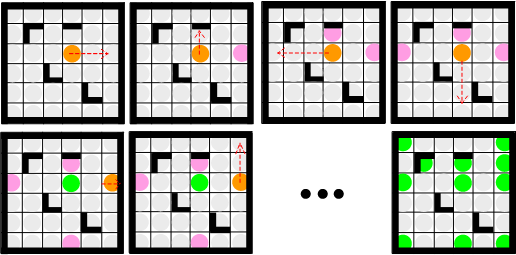
\includegraphics[scale=0.5]{images/bfsRicochet.png}
                    \caption{Visualisation de l'algorithme BFS sur le Ricochet Robots pour un robot}
                \end{figure}
            
        \subsection{Implémentation de l'algorithme A*}
        
            Au début, nous avons implémenté l'algorithme BFS tel quel, car cet algorithme était intéressant et présentait des similarités avec l'algorithme A*. Dans les deux algorithmes, le noeud suivant qui est pris correspond au premier élément d'une liste de noeud à explorer. Cependant, dans l'algorithme BFS, cette liste contient suite à suite les voisins du noeud courant. Ce procédé peut devenir très long et nous nous retrouvions à parcourir des noeuds qui n'étaient pas intéressants à la résolution du problème. Il a donc fallu le modifier pour se rapprocher du modèle de l'algorithme A*.
            
            L'idée est alors d'affecter un coût à chaque noeud, afin de prioriser les noeuds ayant un coût moindre, ce qui nous permettait de nous rapprocher des noeuds solutions. Dans l'algorithme A*, le coût d'un état est alors calculé à la fois par rapport à la profondeur du noeud mais aussi d'une heuristique. Pour que les noeuds soient pris selon le coût du noeud il ne fallait plus ranger la liste des noeuds à visiter selon les éléments voisins. Nous avons donc transformé cette liste en une liste à priorité (PriorityQueue). L'utilité est que chaque nouveau noeud parcouru est choisi comme étant celui qui minimise à la fois la distance parcourue et l'heuristique, qui est le principe même de l'algorithme A*.
            
            Dans le cas du Ricochet Robots, un noeud est représenté par un état du jeu et la flèche par un déplacement d'un robot. Lorsque un robot réalise un déplacement, un nouvel état est créé. L'algorithme vérifie que ce nouvel état ne fait pas parti des noeuds à explorer, ou alors dans le cas ou il est déjà existant, il vérifie si ce nouveau noeud est plus avantageux que celui enregistré ou non. S'il s'agit d'un nouvel état ou d'un noeud avantageux, nous l'ajoutons à la liste des noeuds à explorer, sinon il est ignoré et nous passons à la direction suivante. Lorsque nous ajoutons un élément à la liste des noeuds à explorer, nous ajoutons également dans une HashMap à la fois ce nouveau noeud mais également l'état qui précédait celui-ci, ce qui permet par la suite de retrouver le chemin parcouru qui aura été fait pour atteindre cet état.
            
            Á la fin de ce procédé, nous récupérons l'état gagnant de cette partie. Ensuite, nous recherchons dans la HashMap l'état gagnant (la valeur dans l'HashMap) ainsi que l'état qui a permis d'atteindre cet état (la clé qui est associé à la valeur), puis nous recherchons cet état précèdent et d'où il venait, et ainsi de suite jusqu'à obtenir l'état initial.
            L'ensemble des états successeurs sont ainsi conservés dans une Arraylist de State. Nous inversons ensuite cette ArrayList puisque le cheminement des états est inversé, nous avons commencé de la fin pour aller au départ.
            
            Une fois ce procédé terminé, nous parcourons cet ArrayList et nous récupérons dans chaque état le cheminement des robots qui ont été bougés durant l'état et le cheminement de directions effectuées. Ces deux cheminement sont également conservés dans des ArrayList. Une fois terminé, nous affichons dans le terminal, la couleur du robot à déplacer ainsi que la direction à effectuer à chaque étape afin d'indiquer à l'utilisateur le chemin à parcourir pour atteindre la case d'objectif.
            \newpage
            
            Le code de l'algorithme A* est le suivant:
            
            \scalebox{0.9}{
            \begin{algorithm}[H]%-------------------------------------------
                
                \DontPrintSemicolon
                \KwIn{L'etat initial}
                $etatInitial \gets l'etat\ initial$;
                
                $PriorityQueue<State> frontier \gets new\ PriorityQueue<>()$;
                
            	$HashMap<State,State> cameFrom \gets new\ HashMap<>()$;
            	
            	$HashMap<State,Integer> costSoFar \gets new\ HashMap<>()$;
            	
            	$ArrayList<State> path \gets new\ ArrayList<>()$;
            	
            	$ArrayList<Robot> listRobot \gets new\ ArrayList<>()$;
            	
            	$ArrayList<Deplacement> listDeplacement \gets new\ ArrayList<>()$;
    
    	        $etatInitial.setValCost(0)$;
    	        
    	        $frontier.add(etatInitial)$;
    	        
    	        $cameFrom.put(etatInitial, null)$;
    	        
    	        $costSoFar.put(etatInitial, cout\ de\ l'etat\ initial)$;
        
            	\While{$frontier\ n'est\ pas\ vide$}{
    		
    		        $noeudEnCours \gets frontier.poll()$;
    		
            		\If{$objectif\ atteint$}{
            			$etatFinal \gets noeudEnCours$;
            			
            			$break$;
            		}
            		
            		\For{$chaque\ direction$}{
            			\For{$chaque\ robot$}{
            				$etatSuivant \gets noeudEnCours.etatSuivant(direction, robot)$;
            				
                            $newCost \gets cout\ de\ l'etat\ suivant\ + 1 + heuristique\ de\ l'etat\ suivant$;
            
            				\If{$l'etat\ suivant\ est\ nouveau$ \textsc{or} $le\ cout\ de\ l'etat\ suivant\ est\ plus\ petit\ que\ celui\ de la liste$}{
            					$costSoFar.put(etatSuivant, newCost)$;
            					$etatSuivant \gets cout\ de\ l'etat\ suivant\ + 1$;
            					$frontier.add(etatSuivant)$;
            					$cameFrom.put(etatSuivant, noeudEnCours)$;
            				}
            			}
            		}
            	}
           
    	        $current \gets etatFinal$;
    
            	\While{$current != etatInitial$ {and} $ current != null$}{
            		$path.add(current)$;
            		
            		$current = cameFrom.get(current)$;
            	}
            	\If{$l'etat\ actuel\ existe$}{
            		$path.add(etatInitial)$;
            
            		\For{$chaque\ etat\ du\ chemin$}{
            			$listDeplacement.add(dernier\ deplacement\ de\ l'etat)$;
            			
            			$listRobot.add(dernier\ deplacement\ de\ robot\ de\ l'etat)$;
            		}
            
            		$reverse(listRobot)$;
            		$reverse(listDeplacement)$;
            
            		\For{$chaque deplacement de robot$}{
            			affiche le robot et la direction à effectuer
            		}
            	}
            	\Else{
            		affiche "pas de solution"
            	}
                  \caption{\sc Algorithme A*}
            \end{algorithm}%-------------------------------------------
            }
            
    \subsection{Mise en place de l'heuristique}
    
        Pour que l'algorithme A* soit opérationnel, cet algorithme a besoin d'une heuristique. L'heuristique permet d'aller plus rapidement vers la solution, et ainsi permet d'éviter d'explorer des noeuds qui n'ont pas d'intérêt à être visité.
        Parmi les heuristiques existants, le plus connu est celui du "vol d'oiseau". Cet heuristique permet de calculer la distance du pion actuel par rapport à l'objectif et ainsi, plus la distance est petite, plus le coût sera moindre et plus l'état sera priorisé. Par exemple dans l'image ci-dessous, dans un déplacement d'une case par une case, le noeuds explorés se dirigent directement vers la cible puisque que ce sont des états où le jeton est le plus proche de la solution, la distance est plus petite en allant directement vers sa cible.
        
    
        La mise en place de cet heuristique permet une réelle optimisation. Nous pouvons ainsi le voir sur cette même image l'importance de l'heuristique.
        
           \begin{figure}[H]
                \centering
                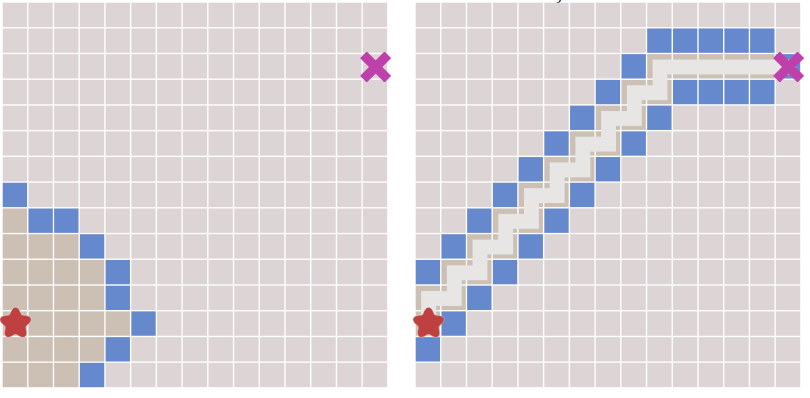
\includegraphics[scale=0.75]{images/2.png}
                \caption{image\cite{redblob} sans et avec heuristique après 23 noeuds explorés }
            \end{figure}
            
        Cependant, ce type d'heuristique n'est pas adapté pour le ricochet robot, puisque le plateau n'est pas construit selon le modèle d'une géométrie standard comparé a une map par exemple. Le fait de se rapprocher de la case d'objectif ne permet pas forcément de récupérer plus rapidement le jeton. Souvent, il est nécessaire de s'éloigner du jeton pour mieux se rapprocher de celui-ci.
        
        Nous avons donc mis en place une carte heuristique. La carte heuristique du ricochet robots consiste à donner à chaque case une valeur heuristique égale au nombre minimum de rebond qu'il faut faire pour atteindre l'objectif. Pour construire cette carte, il faut partir de la fin :
        
        \begin{enumerate}
            \item Toutes les cases qui sont à la verticale ou l'horizontale de  l'objectif sans être bloquées par un mur ont une heuristique de 1.
            \item Toutes les cases qui sont à la verticale ou l'horizontale d'une case possédant une heuristique de 1 et qui ne possèdent pas encore d'heuristique (ont une heuristique de -1) sont à une heuristique de 2.
            \item Toutes les cases qui sont à la verticale ou l'horizontale d'une case possédant une heuristique de 2 et qui ne possèdent pas encore d'heuristique (ont une heuristique de -1) sont à une heuristique de 3.
            \item Toutes les cases qui sont à la verticale ou l'horizontale d'une case possédant une heuristique de 3 et qui ne possèdent pas encore d'heuristique (ont une heuristique de -1) sont à une heuristique de 4.
            \item Et ainsi de suite jusqu'à ce que toutes les cases du plateau qui sont accessibles aux robots aient une heuristique différente de -1.
        \end{enumerate}
        
         \begin{figure}[H]
            \centering
            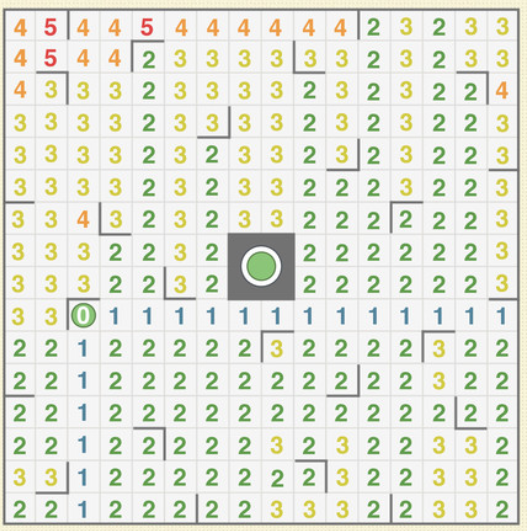
\includegraphics[scale=0.6]{images/mapHeuristique.PNG}
            \caption{Exemple de carte heuristique pour le Ricochet Robots\cite{heurist}}
        \end{figure}
        
        Ainsi l'heuristique d'un état correspond à la valeur d'heuristique de la case sur laquelle se trouve le robot de la couleur de l'objectif.
        
        L'heuristique doit être recalculé après chaque déplacement puisque le moindre mouvement d'un autre robot peut avoir un réel impact sur la partie, qui fausse la valeur de l'heuristique de la case puisque cet autre robot peut à la fois bloquer le chemin vers la solution ou bien favoriser le ricochet du robot.
        
\newpage %%%%%%%%%%%%%%%%%%%%%%%%%%%%%%%%%%%%%%%%%%%%%%%%%%%%%%%%%%%%%%%%%%%%%%%%%%%%%%%%%%%%%%%%%%%%%%%%%%%%%%%%%%%%%%%%%%%%%%%%

\section{Utilisation de l'application}
    \subsection{Lancement du programme}
        Le lancement du jeu se fait par l'exécution du script de compilation, c'est-à-dire en réalisant la commande suivante à la racine du projet:
        \lstinputlisting[firstline=1,lastline=1,numbers=none]{code/compile.sh}
        Le lancement peut également se faire en cliquant directement sur le ficher "launcherBuild.sh", qui exécute la commande indiquée ci-dessus.
        Si nous ne fournissons pas d'arguments à cette commande, alors la taille de la fenêtre sera par défaut de 980x980 pixels. Si nous ajoutons comme argument par exemple 300 comme ci-dessous, alors la fenêtre fera du 300x300 pixels au lancement du jeu.
        \lstinputlisting[firstline=2,lastline=2, numbers=none]{code/compile.sh}
        
        Le contenu de la fenêtre (le plateau, les robots et les autres éléments visuels relatifs au jeu) sont alors adaptés selon la taille de la fenêtre.
        
        \begin{figure}[H]
            \centering
            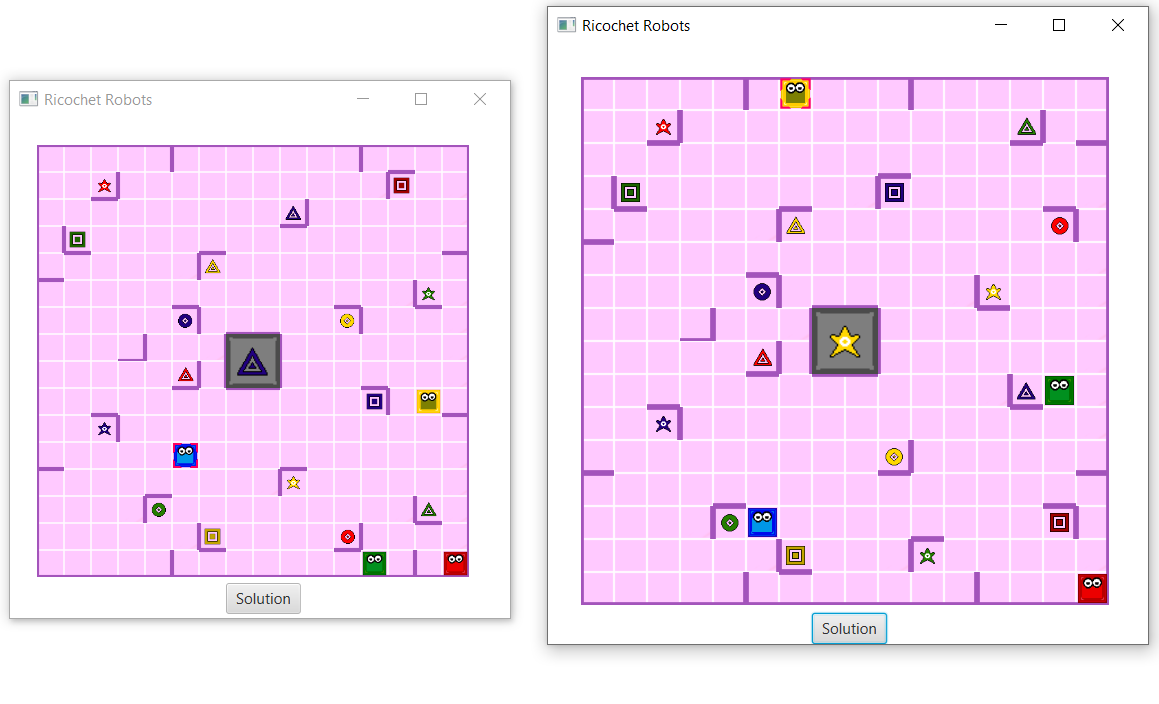
\includegraphics[scale=0.5]{images/dimensionDifferente.PNG}
            \caption{Deux lancements avec 500px (à gauche) et 600px (à droite)}
        \end{figure}
        
    \subsection{Jouabilité}
        Au lancement, nous avons un fenêtre affichant un plateau, quatre robots de différentes couleurs, un jeton au centre correspondant à la case sur laquelle le robot de la même couleur doit aller et un bouton "solution" en dessous de ce plateau. 
        
        \begin{figure}[H]
            \centering
            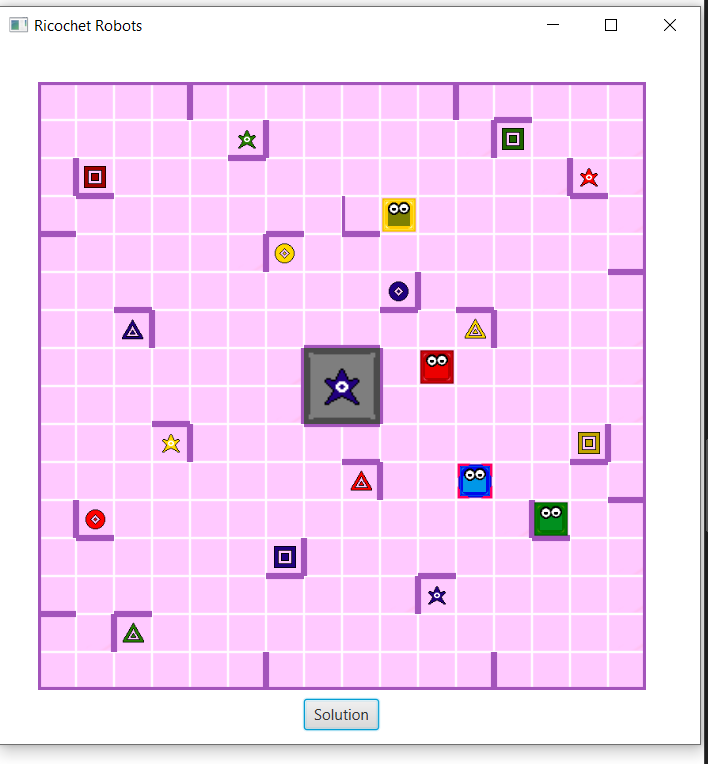
\includegraphics[scale=0.5]{images/fenetre.PNG}
            \caption{Exemple de fenêtre au démarage}
        \end{figure}
        
        
        Le robot pouvant se déplacer est celui qui a la marque de sélection. Sur l'image ci-dessus, il s'agit du robot bleu.
        
        L'utilisateur peut déplacer le robot sélectionné dans les quatre directions (en haut, en bas, à gauche et à droite) avec les touches directionnelles du clavier.
        
        
        L'utilisateur peut sélectionner un autre robot à déplacer en cliquant avec la souris sur cet autre robot. 
        
        \begin{figure}[H]
            \centering
            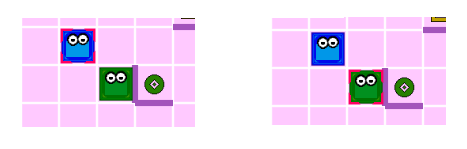
\includegraphics[]{images/selectionRobot.PNG}
            \caption{Avant et après clic sur le robot vert. Le robot vert peut désormais être déplacé}
        \end{figure}
        
        Lorsque le robot atteint la case d'objectif, le socle de ce même robot se positionne sur la case d'objectif, les autres robots retournent sur leur socle et un nouveau jeton est tiré aléatoirement au centre du plateau, désignant ainsi la nouvelle case à aller.
        
        \begin{figure}[H]
            \centering
            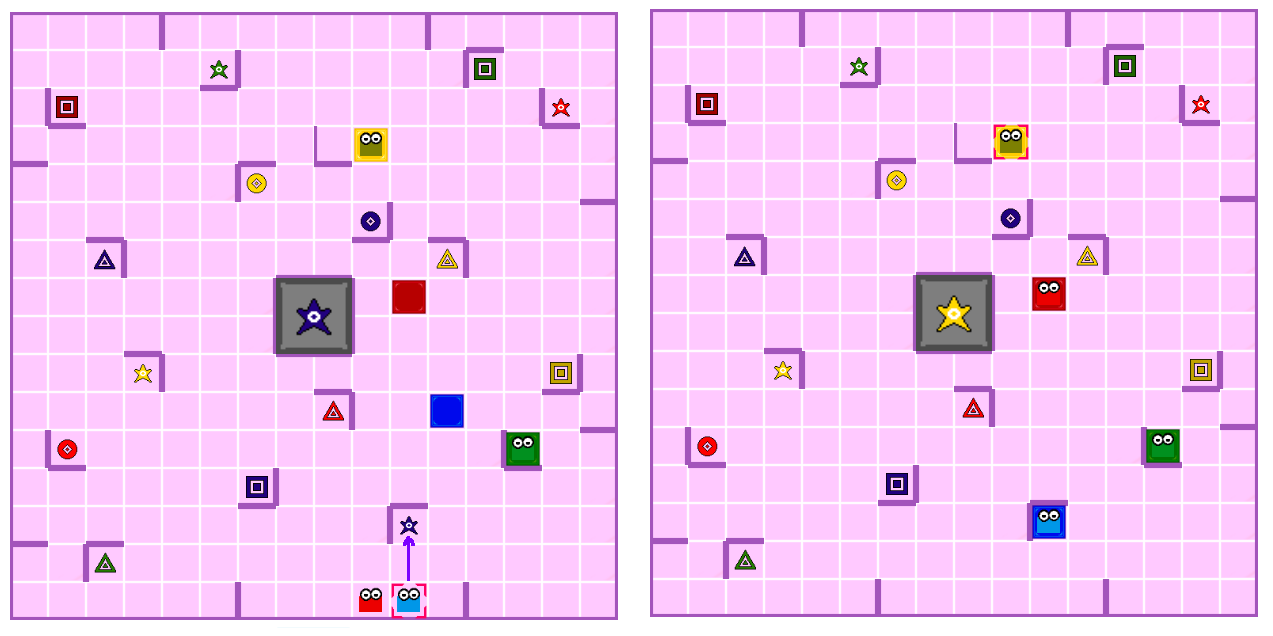
\includegraphics[scale=0.5]{images/objectifAtteint.PNG}
            \caption{Avant et après mouvement pour atteindre l'objectif}
        \end{figure}

    \subsection{Lancement de l'algorithme A*}
    
        L'algorithme A* est utilisé dans cette application comme "outil de solution". Lorsque l'on veut savoir les étapes à effectuer pour atteindre l'objectif, l'utilisateur doit cliquer sur le bouton "solution" situé en dessous du plateau de jeu. Il faut ensuite que l'utilisateur regarde le terminal afin de connaître la solution nécessitant le moins de mouvements.
        
        \begin{figure}[H]
            \centering
            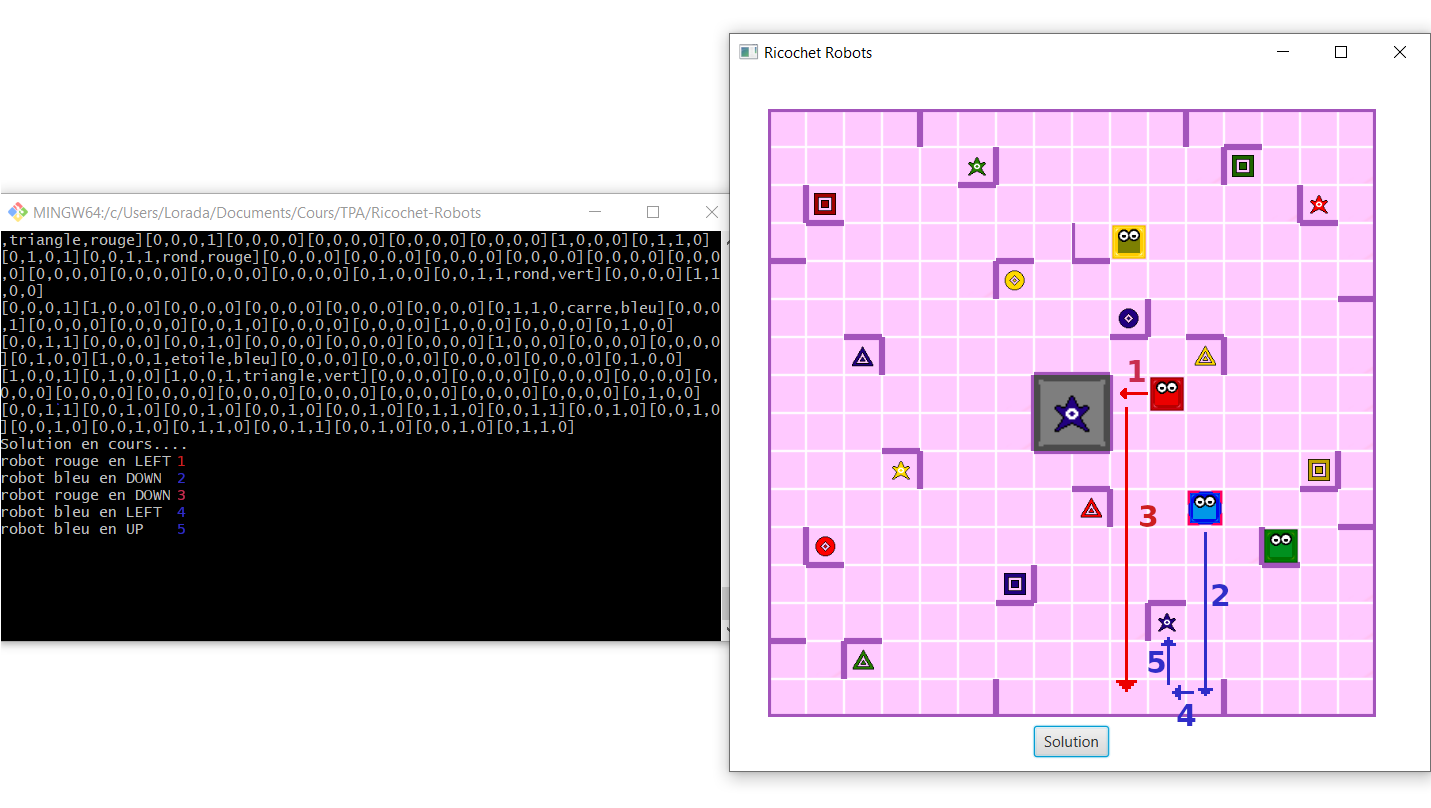
\includegraphics[scale=0.5]{images/mouvementsIa.PNG}
            \caption{Étapes successives indiquées par l'algorithme A*}
        \end{figure}

\newpage %%%%%%%%%%%%%%%%%%%%%%%%%%%%%%%%%%%%%%%%%%%%%%%%%%%%%%%%%%%%%%%%%%%%%%%%%%%%%%%%%%%%%%%%%%%%%%%%%%%%%%%%%%%%%%%%%%%%%%%%

\section{Problèmes rencontrés}

    La partie suivante sera rédigée au nom de Lorada, car elle a été la seule personne à réaliser l'IA.
    \paragraph{}
    Au cours de ce projet, j'ai rencontré différents problèmes que je détaillerai ci-dessous:

    Au niveau de la partie technique, un problème est survenu à partir de l'implémentation de l'algorithme A*, qui m'a pris un certain temps à résoudre. 
    \paragraph{}
    Dans l'algorithme , au moment de comparer deux noeuds afin de savoir si le noeud en cours faisait était déjà présent parmi les noeuds explorés, j'ai utilisé la méthode \textit{contains}.
    Cependant, lors du lancement de l'algorithme, après un certain temps, l'algorithme plantait, en indiquant un StackOverflow comme erreur. J'ai donc regardé la taille du tableau contenant les noeuds restants à explorer au fur et à mesure de l'algorithme et j'ai remarqué que la taille augmentait trop rapidement, comme si tout les noeuds en cours d'exploration s'ajoutaient. J'ai donc regardé le comportement de la méthode \textit{contains}. j'ai remarqué que cette méthode ne marchait pas puisque quelle renvoyait toujours false lors de la vérification d'un nouveau noeud dans la HashMap des noeuds à explorer et ce, même si deux noeuds étaient identiques. Après différentes recherches, j'ai remarqué que j'avais redéfini les méthodes \textit{equals} de l'état, du jeton tiré et de chaque robot, mais que je n'avais pas redéfini la méthode \textit{hashcode} pour que la méthode \textit{contains} fonctionne. J'ai donc regardé le comportement de la méthode \textit{contains} et j'ai remarqué qu'il acceptait certains noeuds mais pas d'autres. J'ai donc sauvegarder dans un fichier une partie des noeuds de la liste des noeuds à explorer, en affichant le hashcode et la position de chaque robot pour chaque état. J'ai remarqué qu'il y avait beaucoup de noeud en plusieurs exemplaires alors que chaque noeud devaient être unique. La méthode \textit{contains} n'était donc pas vraiment fonctionnelle. Au début je me suis demandée si le hashcode n'était pas bon, puisque je n'avais jamais redéfini cette méthode jusqu'à ce moment. Après avoir affiché ce que valait equals et hashcode pour chaque comparaison, les hashcodes étaient tous similaires pour deux états identiques et la méthode équals renvoyait bien true, à la différence de la méthode \textit{contains} qui continuait de me retourner false. Après un long moment de recherche et de tests en vain, j'ai fais en sorte d'agrandir le hashcode de toute les classes ou celui-ci était redéfini, le problème s'est réglé de lui-même, bien que je n'ai pas d'explication à cela.
\newpage %%%%%%%%%%%%%%%%%%%%%%%%%%%%%%%%%%%%%%%%%%%%%%%%%%%%%%%%%%%%%%%%%%%%%%%%%%%%%%%%%%%%%%%%%%%%%%%%%%%%%%%%%%%%%%%%%%%%%%%%

\section{Conclusion}
    \subsection{Conclusion générale}
        Ce projet était très intéressant. Nous ne connaissions pas le Ricochet Robots auparavant et c'était intéressant de se pencher, sur les règles de ce jeu et de le recréer afin de pouvoir y jouer autrement que sous forme physique. Cependant, malgré cette bonne expérience en terme de conception, l'implication faible ou inexistante des personnes du groupe à été un réel frein pour terminer le projet dans les temps et ce malgré la mise en place de différents dispositifs permettant une bonne cohésion de groupe. Le report de la date de rendu a permis de pouvoir corriger les manquements de l'algorithme A*, ce qui n'aurait pu se faire dans les conditions de temps initiales.
    \subsection{Partie personnelles}
        Lorada: Pour ma part, je connaissais déjà le principe de l'algorithme A*, à quoi il servait, mais je ne m'étais jamais réellement penchée dessus et je ne l'avais jamais implémenté auparavant. Bien que j'ai eu quelques difficultés à bien saisir dans le détail certains aspects de cet algorithme, j'ai trouvé très intéressant de le mettre en place dans ce projet.
        
    \subsection{Pistes d'améliorations}
        Bien que nous avons remplis les différents objectifs données pour ce projet, voici une liste non-exhaustive d'améliorations possibles:
        \begin{itemize}
            \item La mise en place du jeton spirale. 
            \item La mise en place d'un système de score.
            \item Une mise en duel entre l'IA et le joueur: si le nombre de mouvements effectués par le joueur est supérieur au nombre minimum de mouvements prévus par l'algorithme A*, alors le joueur gagne un certain nombre de points. Dans l'autre cas, le joueur perd un certain quota de points selon le nombre de déplacements supplémentaires.
            \item L'ajout ou la suppression de robots sur le plateau, bien que ce soit différents du principe de base du Ricochet Robots.
            \item L'ajout d'obstacles (et/ou de malus) ou de bonus sur le plateau. 
            \item Mise en place d'un système de difficulté, rendant plus ou moins punitif les déplacements supplémentaires réalisés par l'utilisateur.
            \item Mise en place du délai imparti à la réflection au nombre de mouvements à faire et un autre délai pour la réalisation du mouvement.
        \end{itemize}
    
\newpage %%%%%%%%%%%%%%%%%%%%%%%%%%%%%%%%%%%%%%%%%%%%%%%%%%%%%%%%%%%%%%%%%%%%%%%%%%%%%%%%%%%%%%%%%%%%%%%%%%%%%%%%%%%%%%%%%%%%%%%%

\bibliographystyle{unsrt}
\bibliography{bibliography}
\end{document}